%% Based on a TeXnicCenter-Template by Gyorgy SZEIDL.
%%%%%%%%%%%%%%%%%%%%%%%%%%%%%%%%%%%%%%%%%%%%%%%%%%%%%%%%%%%%%

%----------------------------------------------------------
%
\documentclass{book} %


\usepackage{amsmath} %
\usepackage{amsfonts} %
\usepackage{amssymb} %
\usepackage{graphicx} %
\usepackage{wrapfig} %
\usepackage{sidecap}
\usepackage{subcaption}


%----------------------------------------------------------
\newtheorem{theorem}{Theorem}
\newtheorem{acknowledgement}[theorem]{Acknowledgement}
\newtheorem{algorithm}[theorem]{Algorithm}
\newtheorem{axiom}[theorem]{Axiom}
\newtheorem{case}[theorem]{Case}
\newtheorem{claim}[theorem]{Claim}
\newtheorem{conclusion}[theorem]{Conclusion}
\newtheorem{condition}[theorem]{Condition}
\newtheorem{conjecture}[theorem]{Conjecture}
\newtheorem{corollary}[theorem]{Corollary}
\newtheorem{criterion}[theorem]{Criterion}
\newtheorem{definition}[theorem]{Definition}
\newtheorem{example}[theorem]{Example}
\newtheorem{exercise}[theorem]{Exercise}
\newtheorem{lemma}[theorem]{Lemma}
\newtheorem{notation}[theorem]{Notation}
\newtheorem{problem}[theorem]{Problem}
\newtheorem{proposition}[theorem]{Proposition}
\newtheorem{remark}[theorem]{Remark}
\newtheorem{solution}[theorem]{Solution}
\newtheorem{summary}[theorem]{Summary}
\newenvironment{proof}[1][Proof]{\textbf{#1.} }{\ \rule{0.5em}{0.5em}}
%----------------------------------------------------------

\usepackage{hyperref}

%----------------------------------------------------------
\begin{document}

% First Page.
\frontmatter
\title{Undergraduate Final Degree Project \\ Design, Development and Implementation of a Multi-Object Tracking Algorithm}
\author{Pablo Ram\'on Soria}
\date{The Date}
\maketitle

%----------------------------------------------------------
% Table of contenst
\tableofcontents

%----------------------------------------------------------
% Preface
\chapter{Preface}

This thesis is the result of a half year research at the Department of Robotics, Vision and Control at the School of Engineering of the University of Seville.

%% 666 TODO: Cosas que han pasado desarrollando

My first word of thanks goes to Bego\~na C. Arrue Ull\'es for helping me not only defining my research question, but also giving me the opportunity to work as an intern in the Department. \\

A Second word of thanks goes to my parents for their motivational support, although I was absent during this time due to studies and works.  \\

Third, I would for my colleague who motivate me to always improve my code and not to settle for the basics.  \\



%----------------------------------------------------------
% Chapter 1. Introduction
\chapter{Introduction}
\section{State of Art}
Computer vision entails mining information from images and video to extract meaningful information. We encounter state-of-the-art computer vision techniques every day-surveillance camera systems \cite{traffic_surveillance_pergamon} \cite{distributed_surveillance} \cite{vehicle_detection}, face detection in our digital cameras, sports analysis, and the recent very popular Kinect system by Microsoft \cite{Kinect_intro}, to name a few. In all of these situations, computer algorithms process images and video to get useful information, so that a human user need not look through, say, hours and hours of surveillance footage. Computer vision research has come a long way over the decades, and today you can take a picture of an object on your cellphone camera and search for it, without typing a word. \\

Particularly, we are focused on improving the computer vision algorithm together with a position estimator for surveillance operations. Task distribution \cite{Coop_Surv_aerial_JJ} \cite{Consensus_reaching_Xiao} \cite{Adaptative_tast_Meuth} \cite{distributed_architecture_Ivan_Maza}  is a key issue in surveillance, many approaches were based on reducing the size and the requirements of the UAVs but increasing the number of these ones. That allows to the system to simplify the tasks and reduce the areas of every vehicle. The Decentralized of the task \cite{descentralized_task_UAV} (That has the associated increasing of the number of the watchers) results in the need of a network that allows to every device to communicate each other and share their information. \\

In regard to the vision algorithm, there are many different method to extract information from every frame. These can be focused in shape segmentation and recognition \cite{shape_using_shape_context} \cite{Vehicle_recog_markov}, color segmentation \cite{} among others, including a combination of them \cite{realtime_signal_recon_shape_color} \cite{signal_recogn_shape_color} \cite{Robust_RT_tracking_color_face_Darrell}.


% 666 TODO....

\section{Objectives}
	The main target of this document is to describe the results of the implemented computer vision algorithm for surveillance that would be run in an embedded computer inside a quadcopter.  \\
	
	Firstly, previously to talk about those results, there's an explanation of each fragment of the algorithm and their equations. \\
	The following chapter, is about the first implementation inside a simulator. The program of the ground station would be the same as the real, but quadcopters and cameras are simulated with V-REP software. \\
	Finally, on the last chapter, the application will be tested inside the embedded computers "Odroid u3" in order to get as much information as possible about speediness of the  algorithm and errors on estimations.

\section{Methodology}
BLA

\section{Structure}
BLA


%% Started the main Content
\mainmatter

%% --> No parts used \part{The First Part}

%----------------------------------------------------------
% Chapter 2. Algorithmcs & Software architecture
\chapter{Algorithmic and Software architecture}
\section{Introduction}
Many approaches of vision systems employing region segmentation \cite{fast_segmentation_Mitra} \cite{fuzzy_segmentation} by color were developed lately. Real-time color based algorithms can be implemented by hardware, but this document describes a fast and non-specific-platform software to deal with it. The software is composed in three parts: Fist one deal with the image, extracting the 2D-objects, this step is called Color Image Segmentation \cite{JamesBruce_CMU_SEG} (or Color Cluster Segmentation: \textbf{CCS} in future mentions); The second one, receive the 2D-object of the previous step and math the objects between two cameras; Afterward the Extended Kalman Filter \cite{GabrielTerejanu_EKF} (\textbf{EKF}), performing with geometric, return the 3D-objects. The last part of the software deal with the communication between both observers in order to arrange the information. Later in section 1.6, a larger explanation of the Software Architecture will be provided.

Previous to the explanation of every step of the algorithm, the following pseudo-code describe the execution of the process.

\begin{algorithm}[hp]
\caption{Tracking algorithm}\label{algorithm_pseudo}
	\begin{algorithmic}[1]
	\Procedure{MainProcess}{}
		\State \Call{setUpEKF}{$params$}
		\State \Call{open}{$camera$}
		\State $\textit{img}  \gets$ \Call{GetImage}{$camera$}
		\If{$\textit{img}$ is empty} 
			\State \Return false
		\EndIf
		
		\State $\textit{objects} \gets$ \Call{Segmentation}{$img$}
		\If{size of $\textit{objects}$} 
			\State \Return false;
		\EndIf
		
		\State $\textit{state} \gets$ \Call{Tracking}{$objects$}
	\EndProcedure
	
	% --------------------------------------------------------------------------
	\Procedure{GetImage}{$VideoSource$}
		\If{$VideoSource$ is open}
			\State $image \gets VideoSource$
			\Return $image$
		\Else $\;$
			\State \Return $Null$
		\EndIf
		
	\EndProcedure
	
	% --------------------------------------------------------------------------	
	\Procedure{Segmentation}{$Image$}
		\If{$Image$ is not HSV}
			\State \Call{convertToHSV}{$Image$}
		\EndIf
		\ForAll{$pixel$ in $Image$}
			\State $pixel \gets$ \Call{conversion}{$pixel$}
		\EndFor
			\State \Return \Call{gatherObjects}{$Image$}
	\EndProcedure
	
	% --------------------------------------------------------------------------		
	\Procedure{Tracking}{$Object$}
		\State $matchedObj \gets$ \Call{Matching}{$Objects$} 
		\If{$matchedObj$ is empty}
			\State \Return $Null$
		\EndIf
		\State $state \gets$ \Call{stepEKF}{matchedObj}
		\State \Return $state$
	\EndProcedure
	
	% --------------------------------------------------------------------------	
	\end{algorithmic}
\end{algorithm}

\section{Segmentation Algorithm}
%----------------------------------------------------------
\subsection{Color Space}
As described previously, in order to extract objects from the scene, the algorithm simplifies the color of every frame in several clusters of colors. To do that, thresholds on color channels were applied. But Firstly the used color space must be defined. \\
RGB is the most common color space, it's composed by three channels (One per color Red, Green and Blue). The main trouble using RGB frames is that objects color can change drastically, and threshold are worst limited (Color depend on three variable so limits between them are not flat surface but curved surface).
Instead of using RGB, in this project, HSV color space are chosen. HSV (Hue, Saturation and Value) has all the color information arrange in only one variable: H or Hue channel. That issue, simplifies the algorithm by making the color separation surfaces flats.  \\

% HSV vs RGB figure
\begin{figure}[h]
	\centering
	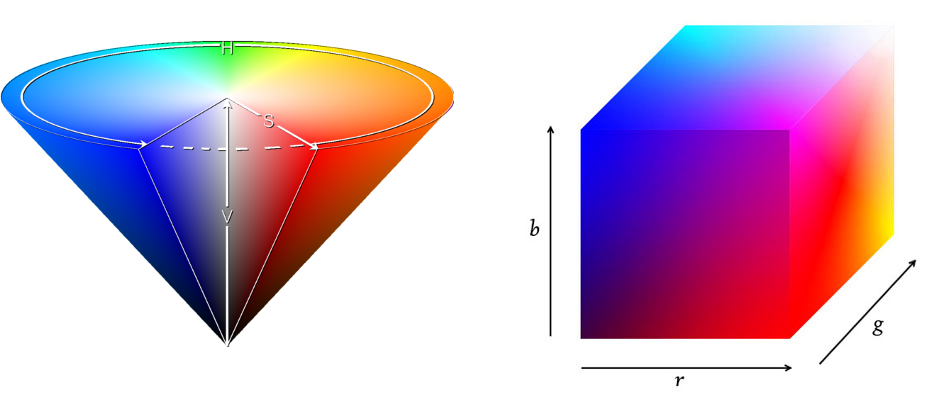
\includegraphics[width=0.75\textwidth,natwidth=944,natheight=400]{../Images/c2/HSV_vs_RGB.png}
	\caption{HSV and RGB spaces of color}
	\label{fig:HSV_vs_RGB}
\end{figure}

%----------------------------------------------------------
\subsection{Pixel Transformation}
Pixel Transformation method refers to the process which takes every single pixel of the image and transform it to a simplified color. That's made by applying a threshold the value of H, S and V channels. \\

\begin{figure}[h]
	\centering
	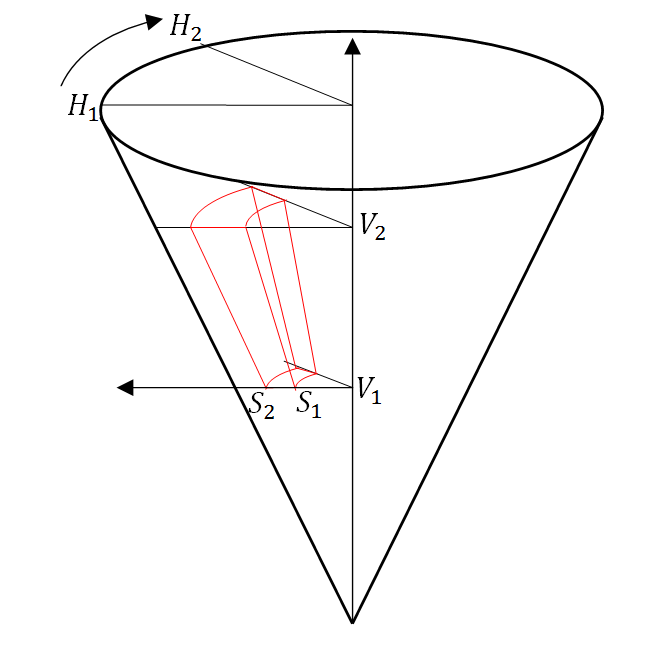
\includegraphics[width=0.5\textwidth,natwidth=659,natheight=659]{../Images/c2/DividingSubSpace.png}
	\caption{Division of subspace}
	\label{fig:DividingSubSpace}
\end{figure}

The common way to apply that threshold if by calling $if...else...$ sentences. But that way is not very efficient because it has got 6 comparison at runtime. Instead, the implementation used on this document, based on CMU algorithm \cite{JamesBruce_CMU_SEG}, consist on boolean thresholds defined at compile-time. This fact reduce considerably the runtime execution. 

Every color space dimension is simplified in $n_i$ clusters ($i = H, S and V$). This decomposition is stored in arrays where every element is a boolean that indicate if the color is in that range. Thus color membership can be computed with three indirection and two bitwise comparison (Between the 3 channels). 

\begin{equation}
\begin{split}
pixel\_col = H\_Range[h] \& \\
S\_Range[s] \& \\
V\_Range[v] 
\end{split}
\end{equation}
	

To illustrate the approach, consider the following example. We divide every channel in ten blocks $(n_H = 10, n_S = 10$ and $n_V = 10)$. So black, for example, might be  represented with the following values in the arrays.

{\centering
\[HRange[10] = \{1, 1, 1, 1, 1, 1, 1, 1, 1, 1\}\]
\[SRange[10] = \{1, 1, 1, 1, 1, 1, 1, 1, 1, 1\}\]
\[VRange[10] = \{1, 1, 1, 0, 0, 0, 0, 0, 0, 0\}\]
} 

Thus, to check if a pixel with color values $(3, 5, 1)$ is a kind of black, it's only necessary to evaluate this expression: 

\[ pixel\_col = HRange[3] \& SRange[5] \& VRange[1] = 1 \& 1 \& 1 = 1 \]

The significant advantage of this approach is that it can evaluate the color membership of multiples color classes simultaneously. Another color example could be blue. In this case the arrays would be:

{\centering
\[HRange[10] = \{0, 0, 0, 0, 1, 1, 1, 0, 0, 0\}\]
\[SRange[10] = \{0, 0, 0, 0, 1, 1, 1, 1, 1, 1\}\]
\[VRange[10] = \{0, 0, 0, 1, 1, 1, 1, 1, 1, 1\}\]
}

Thanks to the parallelism of the bitwise operator, it possible to merge both arrays. So the example with black and blue will have the following array:

{\centering
\[HRange[10] = \{01, 01, 01, 01, 11, 11, 11, 01, 01, 01\}\]
\[SRange[10] = \{01, 01, 01, 01, 11, 11, 11, 11, 11, 11\}\]
\[VRange[10] = \{01, 01, 01, 10, 10, 10, 10, 10, 10, 10\}\] 
} 

Where the high-order bit in each element  of the array represent the $blue$ color and the other one represent the $black$ color. Then, evaluating the previous color $(3,5,1)$ we get: 

\[pixel\_col = HRange[3] \& SRange[5] \& VRange[1] = 01 \& 11 \& 01 = 01\]

which result is black again.

In our implementation we use arrays of bytes of size 36. That allows us to segment every image in 8 different colors with a precision in every channel of $1/36$ defined by the user in code. In conclusion, this method has a high-speed performance but is not adaptable at runtime. \\

Here is the result of applying the algorithm to the well-know picture \textit{Head Scene} of the university of Tsukuba \ref{fig:head_scene_tsukuba_ori} \ref{fig:head_scene_tsukuba_seg}. \\


\begin{figure}[hbp]
	\centering
	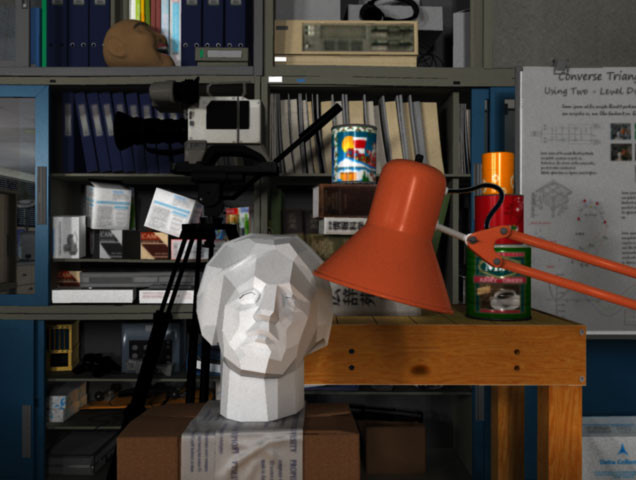
\includegraphics[width=0.4\linewidth]{../Images/c2/head_scene_tsukuba_ori}
	\caption{Original image of the Head Scene}
	\label{fig:head_scene_tsukuba_ori}
\end{figure}

\begin{figure}[htp]
	\centering
	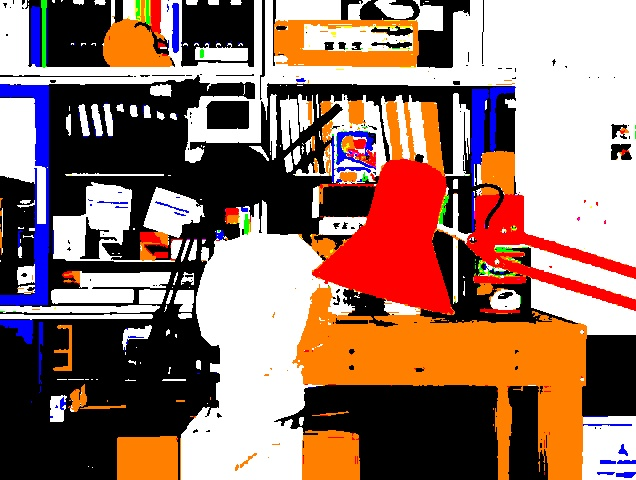
\includegraphics[width=0.4\linewidth]{../Images/c2/head_scene_tsukuba_seg}
	\caption{Segmented image of the Head Scene}
	\label{fig:head_scene_tsukuba_seg}
\end{figure}



%\begin{figure}[h]
%	\centering
%	\begin{subfigure}{0.47\linewidth}
%		\centering
%		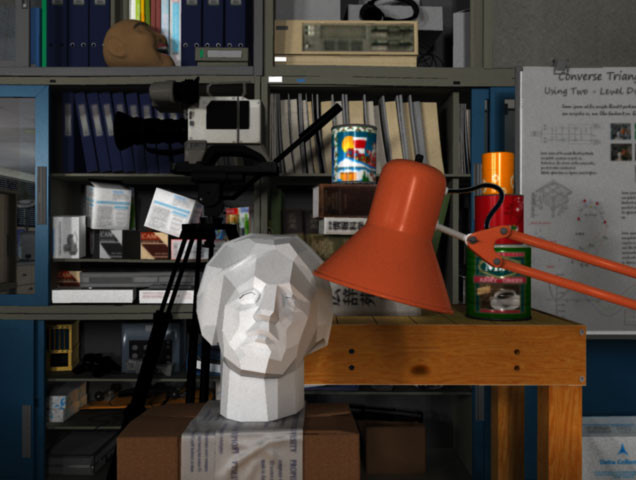
\includegraphics[width=\linewidth]{../Images/c2/head_scene_tsukuba_ori}
%		\caption{Original image of the Head Scene}
%		\label{fig:head_scene_tsukuba_ori}
%	\end{subfigure}
%	~
%	\begin{subfigure}{0.47\linewidth}
%		\centering
%		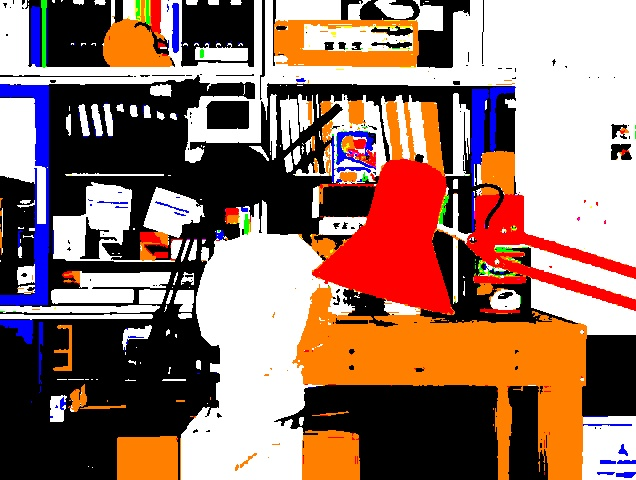
\includegraphics[width=\linewidth]{../Images/c2/head_scene_tsukuba_seg}
%		\caption{Segmented image of the Head Scene}
%		\label{fig:head_scene_tsukuba_seg}
%	\end{subfigure}
%	\caption{Head Scene, University of Tsukuba}
%	\label{fig:Head_Scene}
%\end{figure}



%----------------------------------------------------------
\subsection{Run-length encoding}
Run-length encoding or RLE is a simple form of data compression in which every groups or "runs" of data is compressed by and amount of pairs of data value and count. For example, having the following "runs": \\

\textit{WWWWWWWBBBBBBBBBCCCCCCWWWWWWWWWWWWWWWW} \\

The RLE algorithm will compress it to: \\
\textit{W7B9C6W16}

In this document, RLE is used to reduce image sizes allowing the segmentation algorithm to gather groups of colors and to go over the objects detected in the scene in a simple and fast iteration. \\

This kind of data compress is very useful and effective if the color in the picture is homogeneous. However, if not it could be contra-productive since can make the size of the "runs" grow. Here is an example of both cases: \\

\begin{enumerate}
	\item Homogeneous runs: \textit{WWWWWWWWWWWWWWWWWWWW $\Rightarrow$ W20} \\
	\item Heterogeneous runs: \textit{WAWAWAWAWA $\Rightarrow$ W1A1W1A1W1A1W1A1} \\
\end{enumerate}

%----------------------------------------------------------
\subsection{Object creation}

Once every row of the picture is encoded with RLE it's necessary to connect the regions to extract information about the objects \ref{fig:RLE1}. This is made in two phases. The first one seek per line the adjacent runs with the same color and connect them \ref{fig:RLE2}. Once every line was explored \ref{fig:RLE3}, the second phase look for objects that are splitted due to the first clustering \ref{fig:RLE4}. During the last phase every info is stored in an $"object class"$ that store the size (in pixels), the bouncing box and its centroid.

\begin{figure}
	\centering
	\begin{subfigure}{\linewidth}
		\centering
		\begin{subfigure}{0.4\linewidth}
			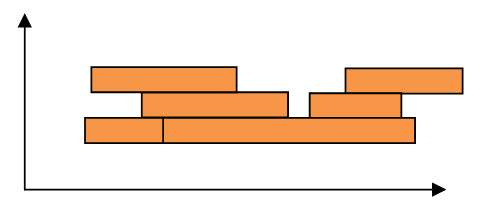
\includegraphics[width=\linewidth]{../Images/c2/RLE1}
			\caption{Runs are disjointed}
			\label{fig:RLE1}
		\end{subfigure}
		%--------------------------------------------------------------------
		\begin{subfigure}{0.4\linewidth}
			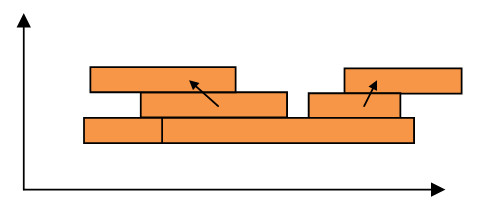
\includegraphics[width=\linewidth]{../Images/c2/RLE2}
			\caption{Vertical scanning result in neighbors clustering}
			\label{fig:RLE2}
		\end{subfigure}
	\end{subfigure}
	~
	\begin{subfigure}{\linewidth}
		\centering
   		\begin{subfigure}{0.4\linewidth}
   			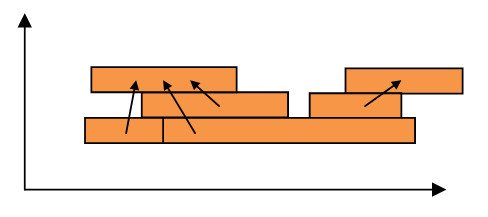
\includegraphics[width=\linewidth]{../Images/c2/RLE3}
   			\caption{All lines joined}
   			\label{fig:RLE3}
   		\end{subfigure}
   		%--------------------------------------------------------------------
   		\begin{subfigure}{0.4\linewidth}
   			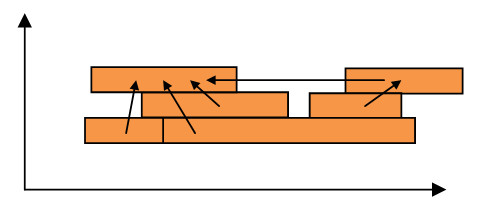
\includegraphics[width=\linewidth]{../Images/c2/RLE4}
   			\caption{Last scanning looking for splitted objects}
   			\label{fig:RLE4}
   		\end{subfigure}
	\end{subfigure}
	\caption{Object creation  from RLEs}
\end{figure}


\section{Matching Algorithm}
The matching consist on link objects between both images. It's an essential step in the algorithm because without step is not possible to track rightly 3D targets.\\

\begin{figure} [htp]
	\centering
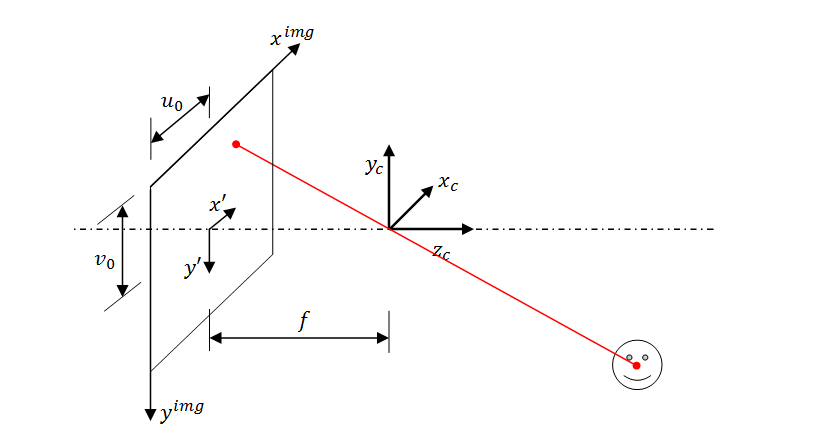
\includegraphics[width=0.75\textwidth,natwidth=544,natheight=388]{../Images/c2/pinhole_model.png} 
	\caption{Pinhole Camera Model}
	\label{fig:Pinhole_Model}
\end{figure}

Firstly, in this article it's assumed that camera's behavior is governed by the pinhole model. According to this and assuming that the X axis of the camera define its the orientation, every space point (X,Y,Z) has the following projection. \\

\begin{equation} \label{eq:pinhole_cam_eq}
\begin{split}
X^{img} = - f*\frac{X}{Z} \\
Y^{img} = f*\frac{Y}{Z}
\end{split}
\end{equation}

Where f is the focal length of the camera; $X^{img}$ and $Y^{img}$ are the projection of the three dimensional point on the camera plane. This equations are in $\mathbb{R}^3$ the equations of 2 planes that cut in one line (The epipolar line). So in conclusion, every segmented object in the camera's images provide a pair of planes (or a single line). Ideally, if the Segmentation had no errors every pair os lines (One per camera for the same target) will cross in a point. However due to errors is almost improbable. That's why the matching algorithm links the objects by minimizing the distance between lines.

\begin{figure}[hp]
\centering
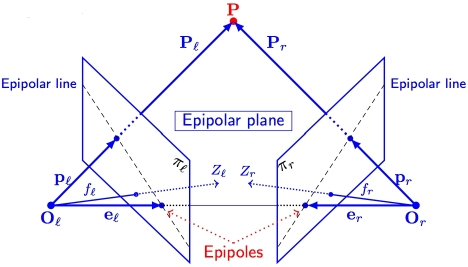
\includegraphics[width=0.75\textwidth,natwidth=468,natheight=267]{../Images/c2/Epipolar_Lines.png}
\caption{Epipolar Lines}
\label{fig:Epipolar_Lines}
\end{figure}

To be precise, the obtained image in the computer hasn't got negative projection. The values on the image are displaced vertically and horizontally. This displacement is stored as the camera�s image centroid or $(u_0, v_0)$. Eventually, equations are: \\

\begin{align}
X^{img} = u_0 - f*\frac{Y}{X}\\
Y^{img} = v_0 + f*\frac{Z}{X}
\end{align}


Due to the noise in the pictures and in the positioning sensors, the pairs of lines would not ever cut. So that, the application minimize the distance between those lines ( \ref{fig:line-min-dist} ). \\
Let be $P_1$ and $P_2$ two points (The first one belong to the line $r_1$ and the second one to $r_2$). This point are defined respectively as: \\

\begin{align}
P_1 = P_1^0 + u_1 * s \\
P_2 = P_2^0 + u_2 * t
\end{align}


Given the definition of these points, the segment $\overline{P_1P_2}$ will be: \\

\begin{equation}
\overline{P_1P_2}=(P_2^0 - P_1^0) + (u_2 * t - u_1 * s)
\end{equation}


The minimal distance is defined as the length of the segment perpendicular to both lines. Mathematically, $\overline{P_1P_2} * u1 = 0$ and $\overline{P_1P_2} * u2 = 0$. Operating with both equations:

\begin{align}
s = \frac{\frac{u_2 * u_2}{u_2 * u_1}*(P_2 - P_1) * u_1 - (P_2 - P_1) * u_2}{\frac{u_2 * u_2}{u_2 * u_1}(u_1 * u_1) - u_1*u_2}	\\
t = \frac{u_1 *_u1 * s - [P_2 - P_1] * u_1}{u_2 * u_1}
\end{align}

Eventually, $dist(r_1,r_2) = norm(\overline{P_1P_2(s,t)})$.

\begin{figure}[htp]
\centering
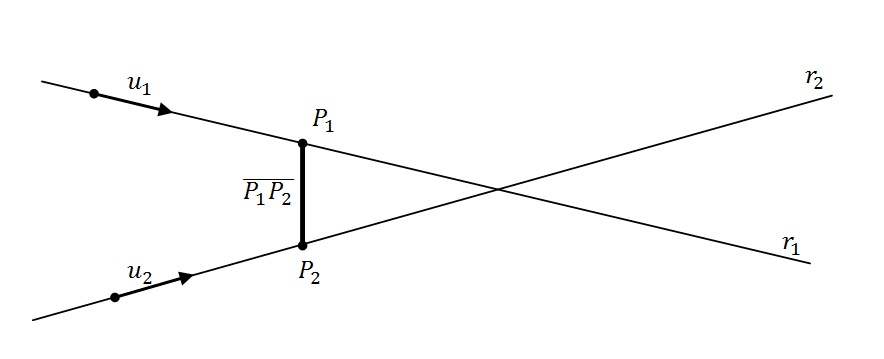
\includegraphics[width=0.7\linewidth]{../Images/c2/line_cut}
\caption{Line minimal distance}
\label{fig:line-min-dist}
\end{figure}




\section{Extended Kalman Filter}
%----------------------------------------------------------
\subsection{System Model} \label{subsec:system_model}

The system consist on a quadrotor with a camera attached and a target that could be on the ground if there is only one vigilant, or "flying" if there's at least two cameras. The coordinates of the point can be described through the camera position thanks to the following equation (Figure: \ref{fig:system_coordinates}).

\begin{equation} \label{eq:system_equation}
P_{obj} = 
	\begin{pmatrix}
	x \\
	y \\
	z \\
	\end{pmatrix}
=
	\begin{pmatrix}
	c_x \\
	c_y \\
	c_z \\
	\end{pmatrix}
+
	\begin{pmatrix}
	r_{11} & r_{12} & r_{13} \\
	r_{21} & r_{22} & r_{23} \\
	r_{31} & r_{32} & r_{33} \\
	\end{pmatrix}
*
	\begin{pmatrix}
	x_c \\
	y_c \\
	z_c \\
	\end{pmatrix}
\end{equation}

\begin{figure}[h]
\centering
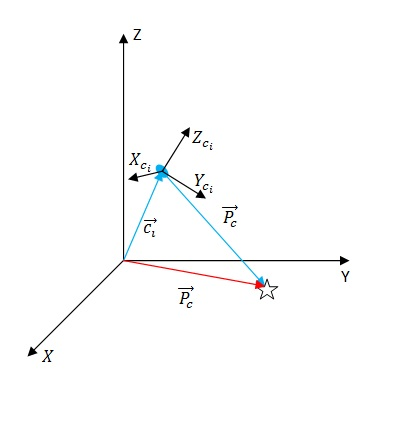
\includegraphics[width=0.5\linewidth]{../Images/c2/system_coordinates}
\caption[System Coordinates]{System Coordinates}
\label{fig:system_coordinates}
\end{figure}


%----------------------------------------------------------
\subsection{Camera Model}
	The model of the camera and its equations had been described on section 2.4. Matching Algorithm.
	
%----------------------------------------------------------
\subsection{Extended Kalman Filter}

The Kalman Filter is an iterative algorithm that obtain an estimation of a lineal dynamic system when sensors has white noise. In this case, the system is non-linear so it's used a variant called Extended Kalman Filter \cite{GabrielTerejanu} (or EKF ). To apply the algorithm it's necessary to use a linealization of the known system described previously. That means that to apply this EKF we consider only the cinematic (velocities of the objects to update their position).

\begin{equation}
P_{obj} = 
	\begin{pmatrix}
	x_k \\
	y_k \\
	z_k \\
	v^{x}_k \\
	v^{y}_k \\
	v^{z}_k \\
	\end{pmatrix}
=
	\begin{pmatrix}
	1 & 0 & 0 & \Delta{t} & 0 & 0 \\
	0 & 1 & 0 & 0 & \Delta{t} & 0 \\
	0 & 0 & 1 & 0 & 0 & \Delta{t} \\
	0 & 0 & 0 & 1 & 0 & 0 \\
	0 & 0 & 0 & 0 & 1 & 0 \\
	0 & 0 & 0 & 0 & 0 & 1 \\
	\end{pmatrix}
*
	\begin{pmatrix}
	x_{k-1} \\
	y_{k-1} \\
	z_{k-1} \\
	v^{x}_{k-1} \\
	v^{y}_{k-1} \\
	v^{z}_{k-1} \\
	\end{pmatrix}
\end{equation}

Consider the following nonlinear system described by the difference equation and the observation model with additive noise: \\

\begin{gather}
x_k = f(x_{k-1}) + w_{k-1} \\
z_k = h(x_k) + v_k
\end{gather}

Been $x_k$ the state of the system, $z_k$ the observation state, and $f(�) \& h(�)$ the functions of both systems with their noise $ w_k ; v_k$. \\
Every step of the EKF consist on two substeps called "Predictor" and "Corrector":

\begin{itemize}
   \item Predictor Step
		\begin{gather}
			x_k^{f} \approx f(x_{k-1}^{a}) \\
			P_k^{f} = J_f(x_{k-1}^{a}) P_{k-1} J_f^{T}(x_{k-1}^{a}) + Q_{k-1}
		\end{gather}

	\item CorrectorStep
		\begin{gather}
			P_k = (I - K_k J_h(x_k^{f}))P_k^{f} \\
			K_k = P_k^{f} J^{T}_h(x_k^{f}) (J_h(x_k^{f}) P_k^{f} J_h^{T}(x_k ^{f}) + R_k)^{-1} \\
			x_k^{a} \approx x_k^{f} + K_k (z_k - h(x_k^{f}))
		\end{gather}
\end{itemize}

In the previous ecuations, $J_h$ and $J_f$ are the Jacobian matrix of the system and observator. They are can be computed basing on the system and camera model as: \\

\[J_h =  
	\begin{pmatrix}
		\frac{\partial h_1}{\partial x_1} & \dots & \frac{\partial h_1}{\partial x_n} \\
		\vdots & \ddots & \vdots \\
		\frac{\partial h_m}{\partial x_1} & \dots & \frac{\partial h_m}{\partial x_n}
	\end{pmatrix}
\]

And so on with the $ f(�)$ function for the $J_f$ jacobian. Following paragraphs decribes the procedure of acquisition of both jacobians for this specific situation. \\

\begin{equation} \label{eq:observation_equation}
z_k =
	\begin{pmatrix}
		x_{img} \\
		y_{img}
	\end{pmatrix}
\stackrel{\ref{eq:pinhole_cam_eq}}{=}
	\begin{pmatrix}
		f*\frac{y_c}{x_c} \\
		f*\frac{z_c}{x_c}
	\end{pmatrix}
\end{equation}

Getting \ref{eq:system_equation} and isolating the position vector of the target in the camera's base, then is possible to express the observation state in term of real system state.

\begin{equation}
\ref{eq:system_equation} \Rightarrow 
	\begin{pmatrix}
		x_c \\
		y_c \\
		z_c 
	\end{pmatrix}
=
	\begin{pmatrix}
		r_{11} & r_{21} & r_{31} \\
		r_{12} & r_{22} & r_{32} \\
		r_{13} & r_{23} & r_{33}
	\end{pmatrix}
*
	\begin{pmatrix}
		x - c_x \\
		y - c_y \\
		z - c_z
	\end{pmatrix}
\end{equation}

So, individually:

\begin{equation}
\left\{ 
	\begin{aligned}
		x_c = r_{11}(x-c_x) + r_{21}(y-c_y) + r_{31}(z-c_z) \\
		y_c = r_{12}(x-c_x) + r_{22}(y-c_y) + r_{32}(z-c_z) \\
		z_c = r_{13}(x-c_x) + r_{23}(y-c_y) + r_{33}(z-c_z) 
	\end{aligned} \right.
\end{equation}

Introducing this in equation \ref{eq:observation_equation}.

\begin{equation}
z_k =
	\begin{pmatrix}
		-f�\frac{r_{11}(x-c_x) + r_{21}(y-c_y) + r_{31}(z-c_z)}{r_{13}(x-c_x) + r_{23}(y-c_y) + r_{33}(z-c_z)} \\
		f�\frac{r_{12}(x-c_x) + r_{22}(y-c_y) + r_{32}(z-c_z)}{r_{13}(x-c_x) + r_{23}(y-c_y) + r_{33}(z-c_z)}
	\end{pmatrix}
\end{equation}

This observation equation only includes information about one camera, since now, this section splits in two. The first one dedicated to stereo tracking with a pair of non-parallel cameras. And the second one, using only one camera but in order to reduce the number of variables (Unless the EKF will became unstable with this equations, in chapter \ref{chap:c6_conclusions} there is a dissertation about this topic). \\

%%% ------------------------------------------------------------------------------------------------
\subsubsection{Tracking of ground objects}
At this point, we suppose that in world coordinates the $z$ dimension of the target is constant, so the system state will be $x_k = (x, y, v_x, v_y)$. For this reason, $\partial z$ and $\partial v_z$ has no sense. Based on a lineal behavior in the system \ref{subsec:system_model} and on the observation equations \ref{eq:observation_equation}, the following matrix are the ones that define the EKF.

\begin{equation}
J_f = 
	\begin{pmatrix}
			1		&		0		&		\Delta_t	&		0					\\
			0		&		1		&		0					&		\Delta_t	\\
			0		&		0		&		1					&		0					\\
			0		&		0		&		0					&		1
	\end{pmatrix}
\end{equation}

\begin{equation}
J_h = 
	\begin{pmatrix}
		-\frac{r_{11}z_c - r_{13}x_c}{x_c^2} & -\frac{r_{21}z_c - r_{23}x_c}{z_c^2}  & 0 & 0  \\
		\frac{r_{12}z_c - r_{13}y_c}{x_c^2} & \frac{r_{22}z_c - r_{23}y_c}{z_c^2}  & 0 & 0 
	\end{pmatrix}
\end{equation}

Such that, $(x_c, y_c, z_c)$ are related to camera position ob the object, $r_ij$ means the $(i,j)$ element of the rotation matrix of the camera.\\ 

%%% ------------------------------------------------------------------------------------------------
\subsubsection{Stereo Tracking}
At this point, unlike previous section the target can move in three coordinates, so the system state will be $x_k = (x, y, z, v_x, v_y, v_z)$. Based on a lineal behavior in the system \ref{subsec:system_model} and on the observation equations \ref{eq:observation_equation}, the following matrix are the ones that define the EKF.

\begin{equation}
J_f = 
	\begin{pmatrix}
			1		&		0		&		0		&		\Delta_t	&		0					&		0					\\
			0		&		1		&		0		&		0					&		\Delta_t	&		0					\\
			0		&		0		&		1		&		0					&		0					&		\Delta_t	\\
			0		&		0		&		0		&		1					&		0					&		0					\\
			0		&		0		&		0		&		0					&		1					&		0					\\
			0		&		0		&		0		&		0					&		0					&		1
	\end{pmatrix}
\end{equation}

\begin{equation}
J_h = 
	\begin{pmatrix}
		-\frac{r_{11}^{c1}z^{c1}_c - r_{13}^{c1}x^{c1}_c}{{(z^{c1}_c)}^2} & -\frac{r_{21}^{c1}z^{c1}_c - r_{23}^{c1}x^{c1}_c}{{(z^{c1}_c)}^2} & -\frac{r_{31}^{c1}z^{c1}_c - r_{33}^{c1}x^{c1}_c}{{(z^{c1}_c)}^2} & 0 & 0 & 0 \\
		\frac{r_{12}^{c1}z_c^{c1} - r_{13}^{c1}y_c^{c1}}{{(z^{c1}_c)}^2} & \frac{r_{22}^{c1}z_c^{c1} - r_{23}^{c1}y_c^{c1}}{{(z^{c1}_c)}^2} & \frac{r_{32}^{c1}z_c^{c1} - r_{33}^{c1}y_c^{c1}}{{(z^{c1}_c)}^2} & 0 & 0 & 0 \\
		
		-\frac{r_{11}^{c2}z^{c2}_c - r_{13}^{c2}x^{c2}_c}{{(z^{c2}_c)}^2} & -\frac{r_{21}^{c2}z^{c2}_c - r_{23}^{c2}x^{c2}_c}{{(z^{c2}_c)}^2} & -\frac{r_{31}^{c2}z^{c2}_c - r_{33}^{c2}x^{c2}_c}{{(z^{c2}_c)}^2} & 0 & 0 & 0 \\
		\frac{r_{12}^{c2}z_c^{c2} - r_{13}^{c2}y_c^{c2}}{{(z^{c2}_c)}^2} & \frac{r_{22}^{c2}z_c^{c2} - r_{23}^{c2}y_c^{c2}}{{(z^{c2}_c)}^2} & \frac{r_{32}^{c2}z_c^{c2} - r_{33}^{c2}y_c^{c2}}{{(z^{c2}_c)}^2} & 0 & 0 & 0 \\
				
	\end{pmatrix}
\end{equation}

And as above, $(x_c, y_c, z_c)$ are related to camera position of the object, $r_ij$ means the $(i,j)$ element of the rotation matrix of the camera and $c_i$ superindex means related to camera i.


\section{Communication}
BLA

\section{Architecture}
On previous sections every fragment of the system was described. Figure \ref{fig:System_Architecture} give a look to the common architecture of the system. It's composed for a number of quads rotors that send to the computer related to their cameras position of the objects that the detect through a simple server-client communication by WiFi wireless devices.

% System architecture image
\begin{figure}[hb]
	\centering
	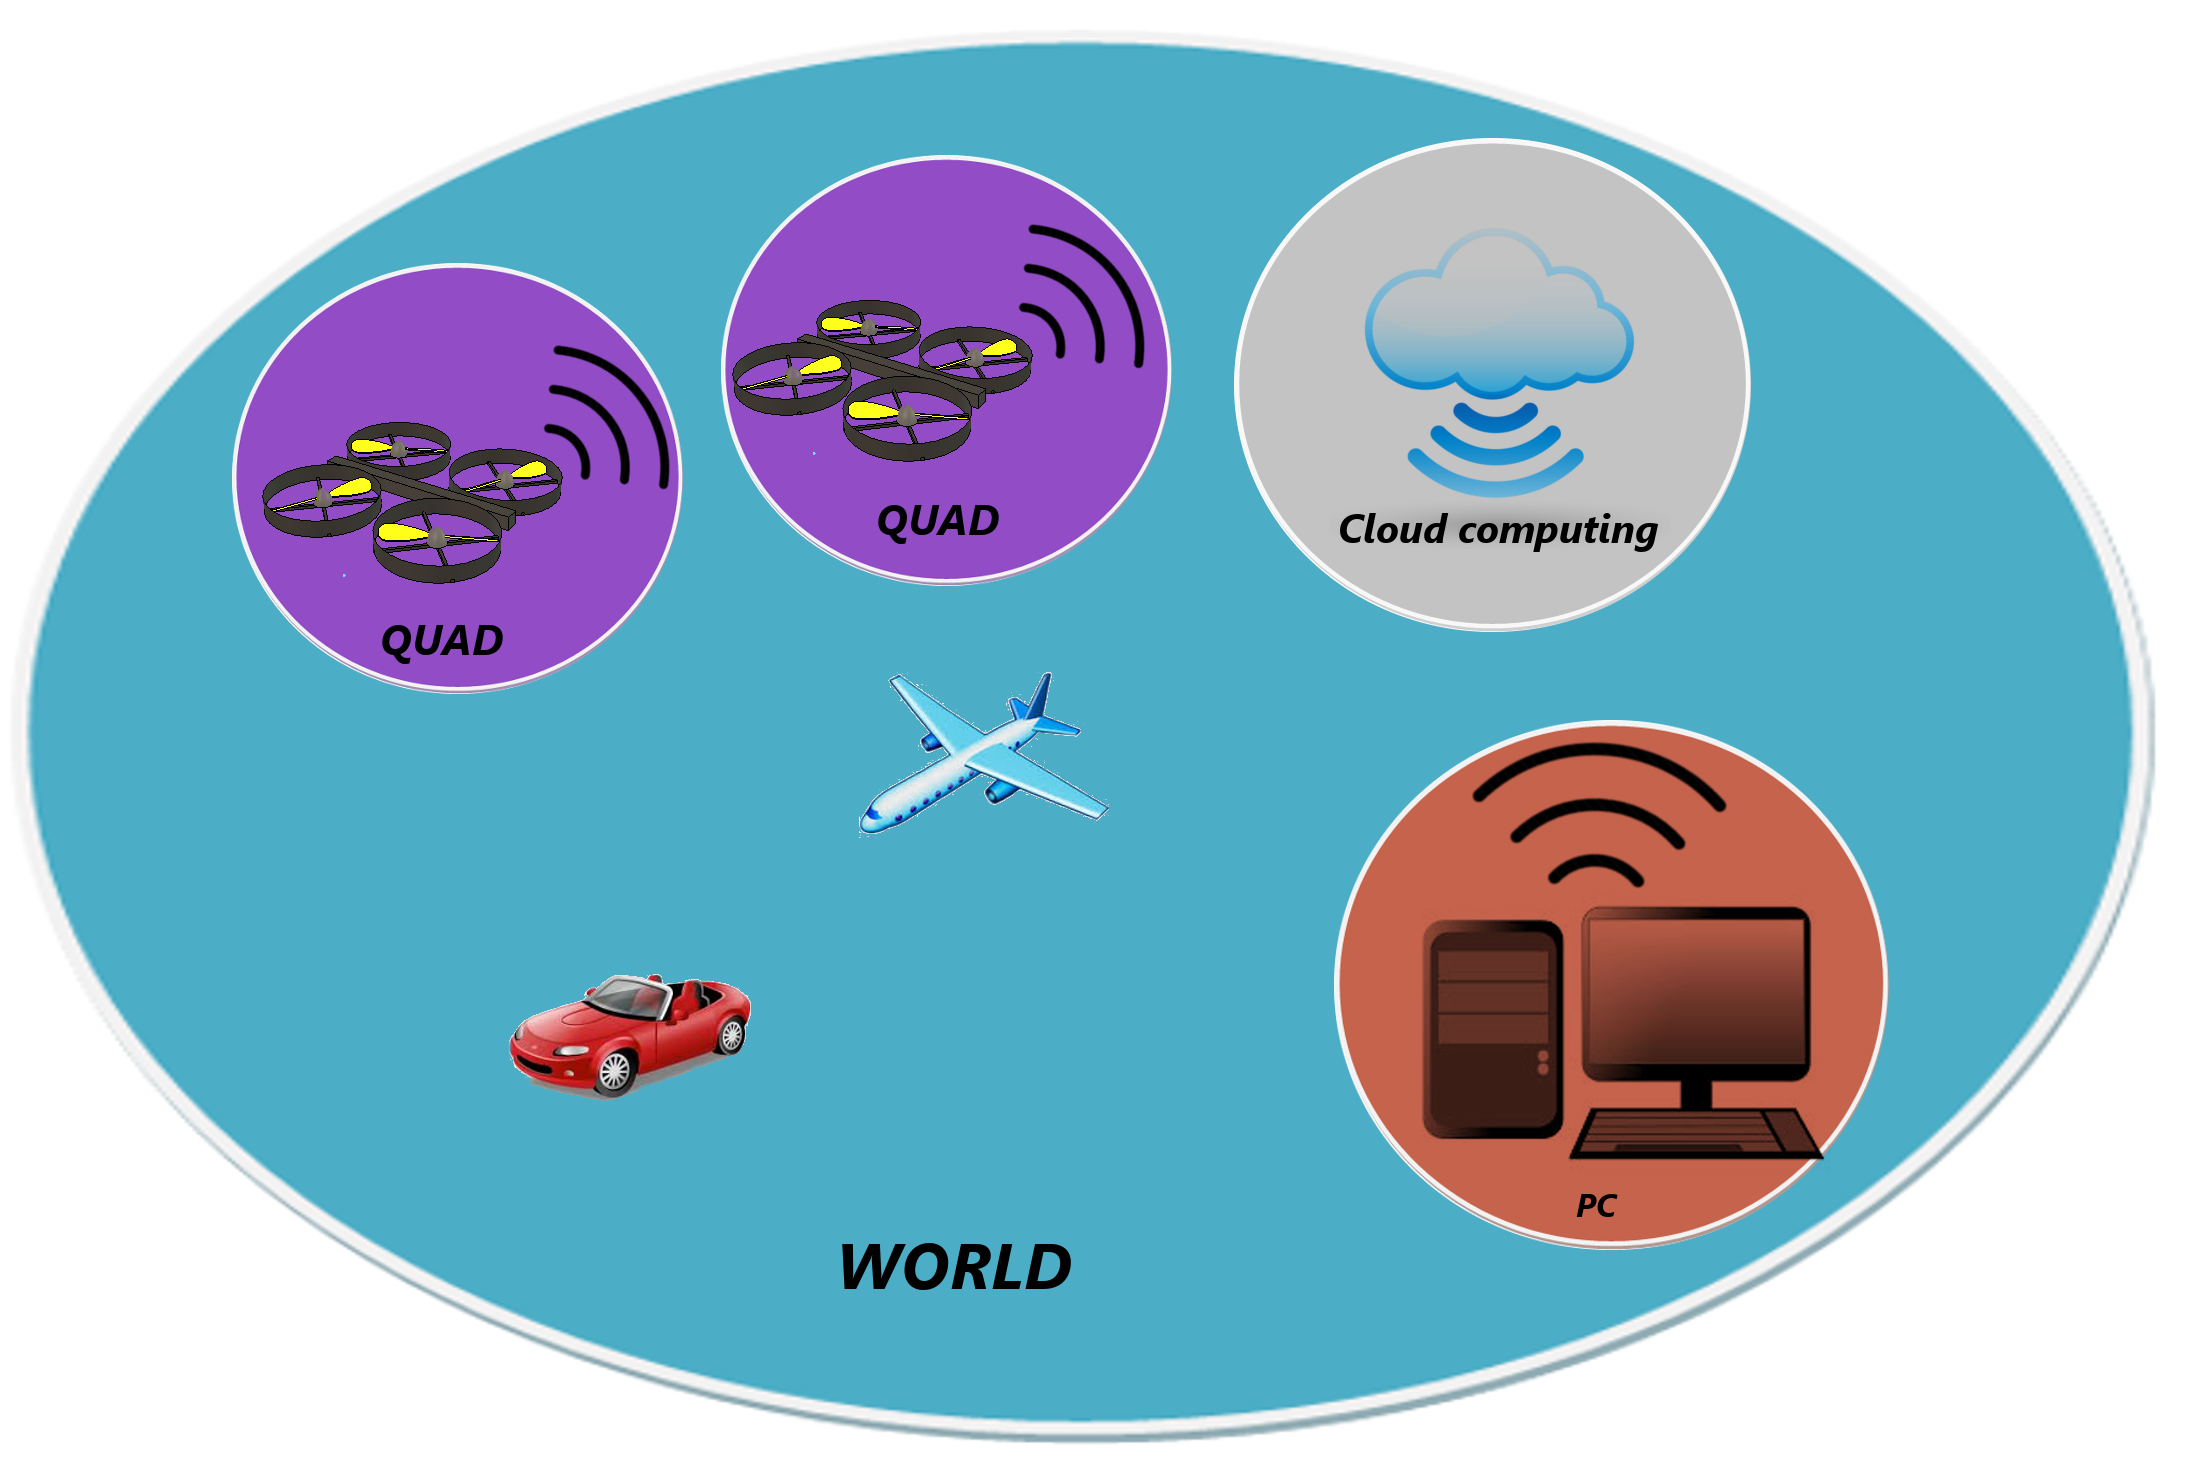
\includegraphics[width=0.50\textwidth,natwidth=220,natheight=1467]{../Images/c2/Architecture.png}
	\caption{System Architecture}
	\label{fig:System_Architecture}
\end{figure}



%----------------------------------------------------------
% Chapter 3. Simulation on VREP 
\chapter{Simulation on VREP}
\section{Introduction}
The robot simulator V-REP, with integrated development environment, is based on a distributed control architecture: each object/model can be individually controlled via an embedded script, a plugin, a ROS node, a remote API client, or a custom solution. This makes V-REP very versatile and ideal for multi-robot applications. Controllers can be written in C/C++, Python, Java, Lua, Matlab, Octave or Urbi. \\

Previous to real implementation, in order to probe the effectiveness of the vision algorithm and the complete tracking architecture, the situation was simulated in this program. In this chapter will be described the process and the results of this simulations.

\subsection{The GUI}

In the following picture (Picture: \ref{fig:VREP_GUI}) shows the common user's interface of the simulator. At the top, there is the common edit buttons and camera movement through the scene. Also at the top on the right are the basic simulate configuration and buttons.

Some pre-created objects can be found in the model browser menu. There are a huge variety of mobile and fixed robots with their own AI and behavior integrated. This acts can be modified or amplified adding plugins or scripts as described previously.

Finally in the center of the interface the interface is the scene visualization. Objects are organized in the hierarchy menu on the left side of the scene.

\begin{figure}
	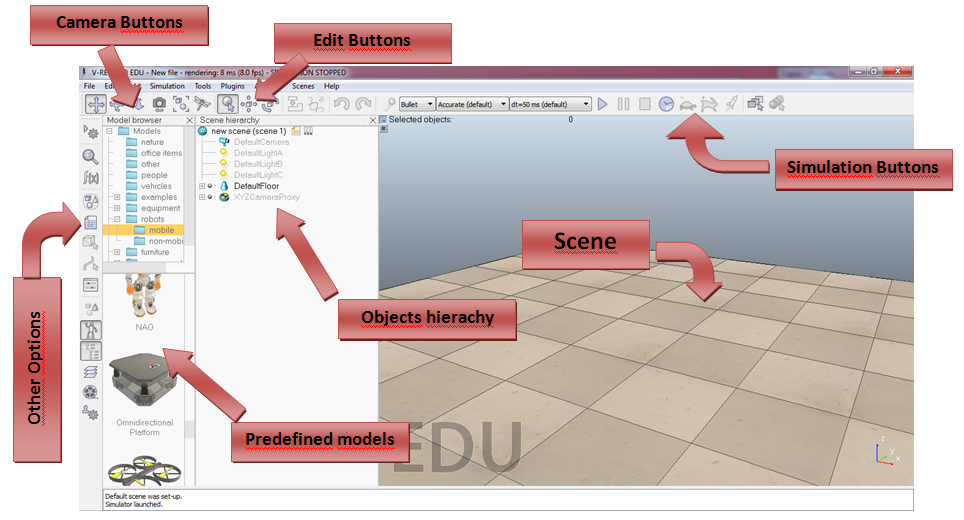
\includegraphics[width=\textwidth,natwidth=964,natheight=520]{../Images/c3/vrep_main.png}
	\caption{V-REP GUI}
	\label{fig:VREP_GUI}
\end{figure}




\section{Implementation in VREP program}
%-------------------------------------------------------------------------------------------------------
%-------------------------------------------------------------------------------------------------------
%-------------------------------------------------------------------------------------------------------
\subsection{Structure of section}
Every section of this chapter is a simulation of the future application. Every simulation is has his own scene (Showed in this document with some images, for example as in Figure: \ref{fig:VREP_scene_example}). This scenes contains the requited quadrotors and targets in order to test the behavior previous real results. Results of vision algorithm is showed in the vrep console(Figure: \ref{fig:Ground_Tracking_VREP_Console}). \\

\begin{figure}[h]
	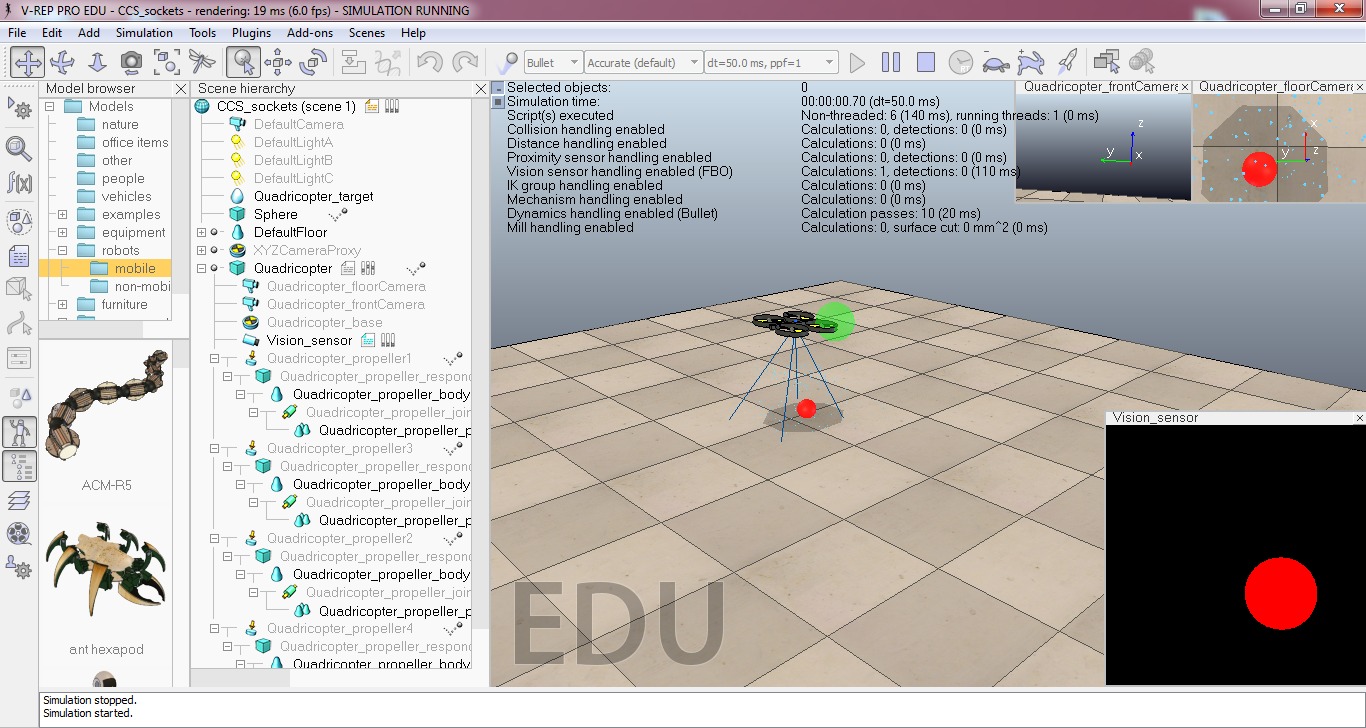
\includegraphics[width=0.7\textwidth,natwidth=1366,natheight=728]{../Images/c3/ground_tracking_scene.png}
	\caption{Ground Tracking Scene}
	\label{fig:VREP_scene_example}
\end{figure}

\begin{figure}[h]
	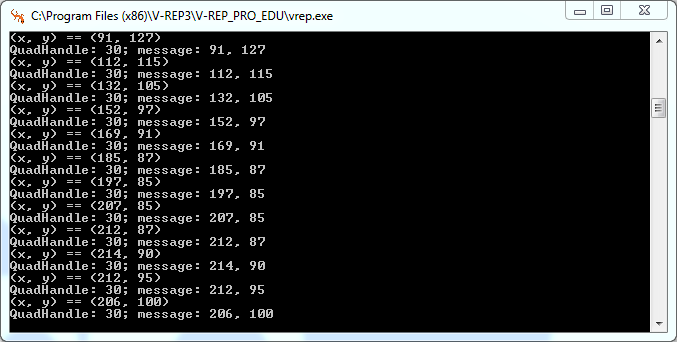
\includegraphics[width=0.7\textwidth,natwidth=677,natheight=342]{../Images/c3/ground_tracking_vrep_console.png}
	\caption{Ground Tracking V-REP Console}
	\label{fig:Ground_Tracking_VREP_Console}
\end{figure}

There is another component in the simulations, the ground station, with the aim to make the most realistic simulations, this ground station is exactly the same as real test ground station. This is possible due to the abstraction of the communication through sockets. The ground station has a simple interface to get some information about the progress. An example of this interface is shown in the Figure: \ref{fig:Ground_Tracking_Server_Console}.

\begin{figure}[h]
	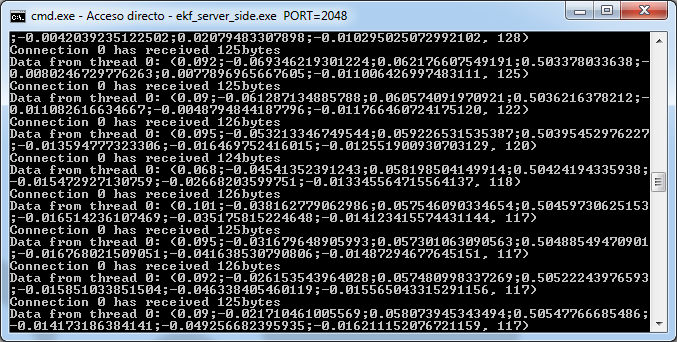
\includegraphics[width=0.7\textwidth,natwidth=677,natheight=342]{../Images/c3/ground_tracking_server_console.png}
	\caption{Ground Tracking Server Console}
	\label{fig:Ground_Tracking_Server_Console}
\end{figure}

Both ground station and objects in the simulation generate a LOG in order to analyze afterwards the results.

%-------------------------------------------------------------------------------------------------------
%-------------------------------------------------------------------------------------------------------
%-------------------------------------------------------------------------------------------------------
\subsection{Simulation 1 - Simple ground camera tracking. Vertical camera}
\subsubsection{Set up}
This Scene has basically one quad rotor and one target (Figure: \ref{fig:VREP_scene_example}). The Red sphere is moving on the floor (Describing a circle) while the quad's camera captures pictures and the on board (simulated) computer process it and command the drone in order to follow the target. In this simulation the camera is facing the ground (Figure: \ref{fig:ground_tracking_scene_vertical}).

\begin{figure}[h]
	\centering
	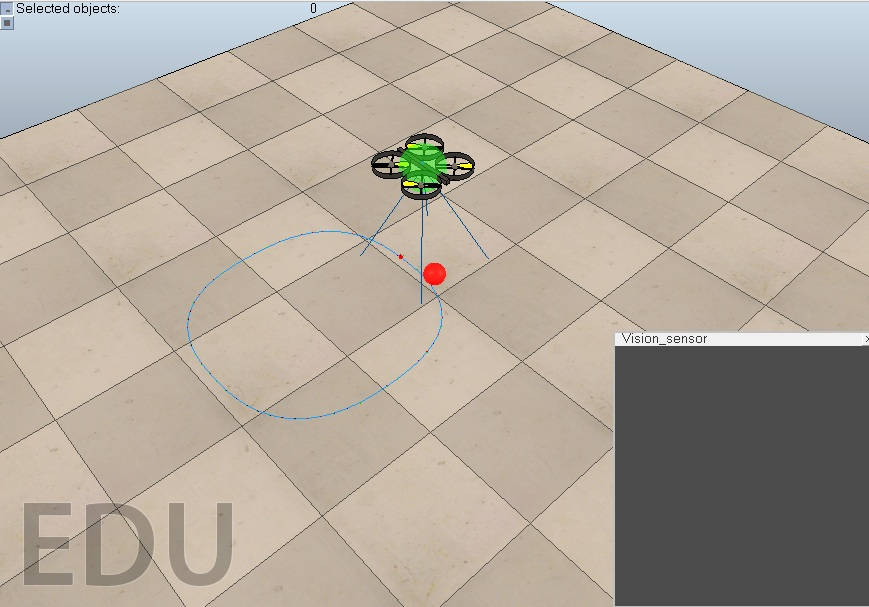
\includegraphics[width=0.7\linewidth]{../Images/c3/ground_tracking_scene_vertical}
	\caption{Ground tracking - Oblique Camera}
	\label{fig:ground_tracking_scene_vertical}
\end{figure}

\subsubsection{Test and results}

	In this test the maximum error (That is about 4.6 cm) is at the beginning of the simulation Due to the initial state of the EKF. Lately the this error is reduced to $\sim$ 1 cm. The fist figure (\ref{fig:sim1_traj_ori} and \ref{fig:sim1_traj_track}) that contains 2 pictures, shows X and Y coordinate of the a) real trajectory and b) the results of EKF algorithm. The last figure of this simulation shows the 3D path that was described by the target (Blue line) and the tracked trajectory (Red line); Figure \ref{fig:sim1_traj_both_3d}.
	
\begin{figure}[h]
	\centering
	\begin{subfigure}[b]{0.4\linewidth}
		\centering
		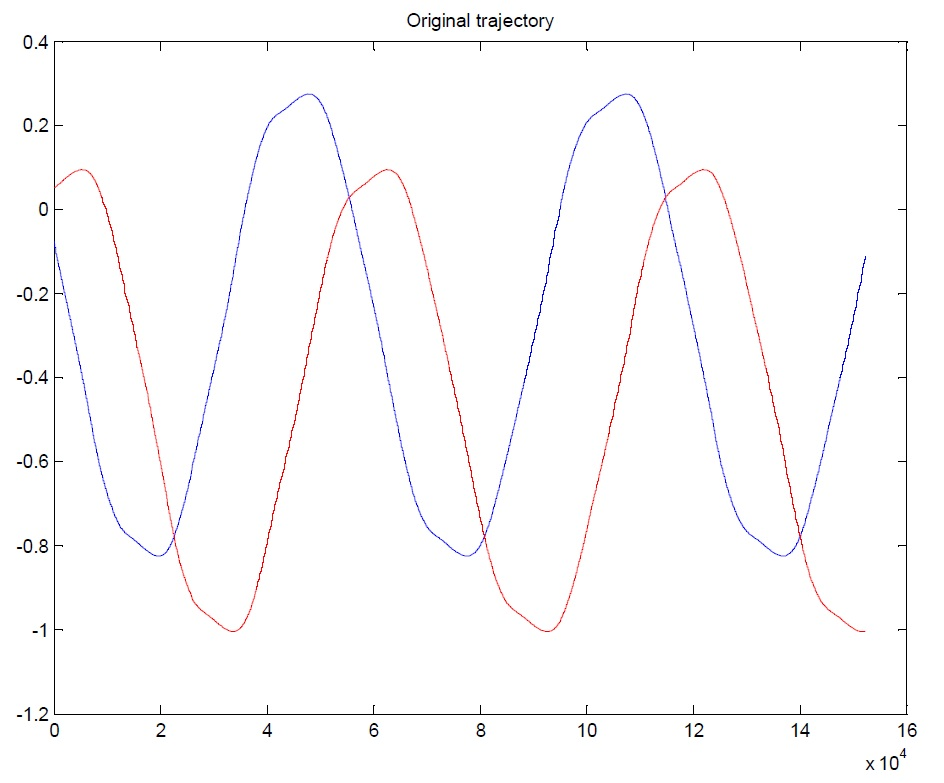
\includegraphics[width=\linewidth]{../Images/c3/sim1_traj_ori}
		\caption{Ground tracking - Original trajectory}
		\label{fig:sim1_traj_ori}
	\end{subfigure}
	~
	\begin{subfigure}[b]{0.4\linewidth}
		\centering
		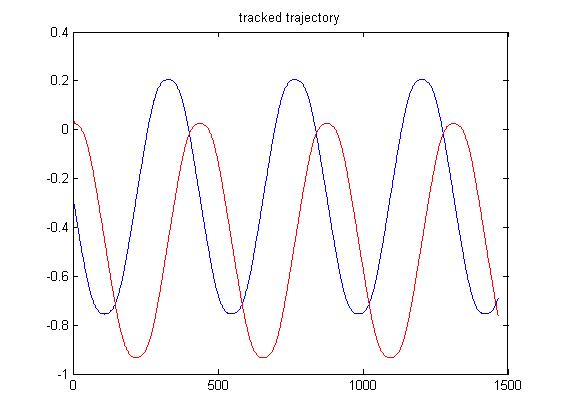
\includegraphics[width=\linewidth]{../Images/c3/sim1_traj_track}
		\caption{Ground tracking - Tracked trajectory}
		\label{fig:sim1_traj_track}
	\end{subfigure}

\end{figure}


\begin{figure}[h]
\centering
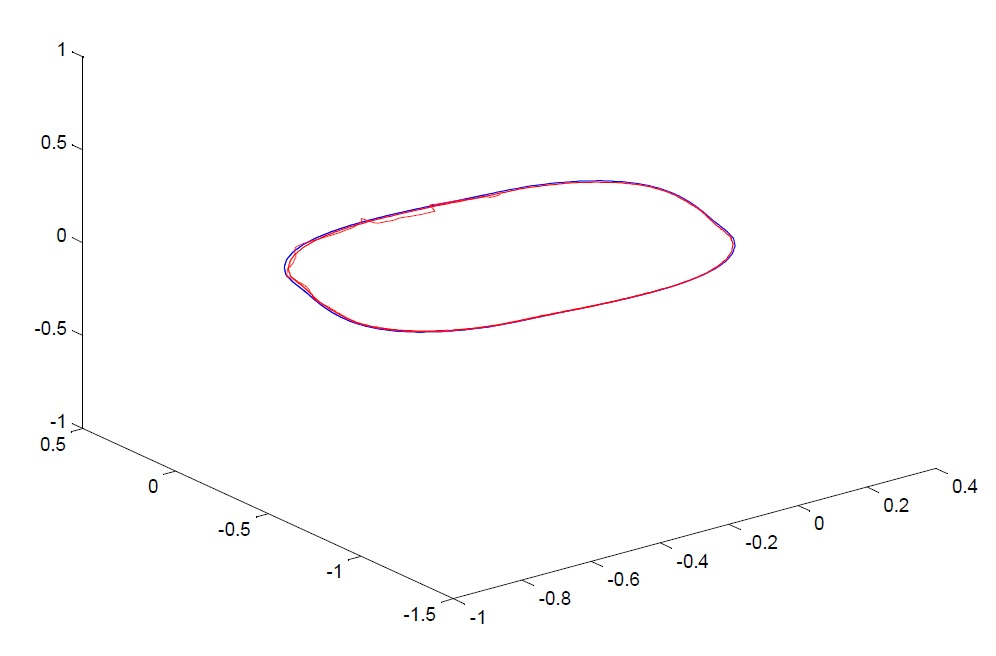
\includegraphics[width=0.7\linewidth]{../Images/c3/sim1_traj_both_3d}
\caption{Ground tracking - Oblique Camera - 3D trajectory}
\label{fig:sim1_traj_both_3d}
\end{figure}




%-------------------------------------------------------------------------------------------------------
%-------------------------------------------------------------------------------------------------------
%-------------------------------------------------------------------------------------------------------
\subsection{Simulation 2 - Simple ground camera tracking. Oblique camera}
\subsubsection{Set up}
This Scene has basically one quad rotor and one target. The Red sphere is moving on the floor (Describing a curve) while the quad's camera captures pictures and the on board (simulated) computer process it and command the drone in order to follow the target. In this case, the camera is not facing directly the ground, now it's oblique (45 degrees from the previous; Figure: \ref{fig:ground_tracking_scene_oblique}). At this experiment, the speed of the target was increased.

\begin{figure}[h]
	\centering
	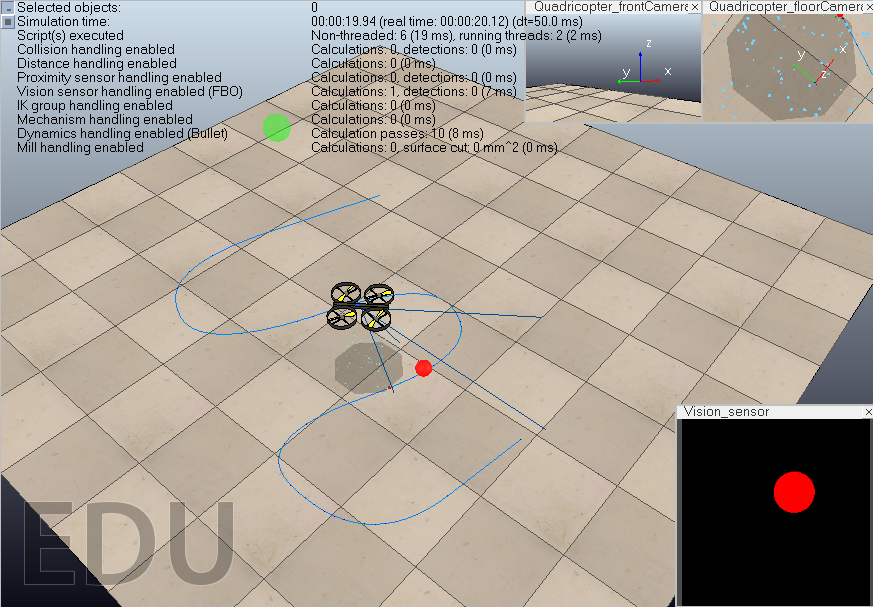
\includegraphics[width=0.7\linewidth]{../Images/c3/ground_tracking_scene_oblique}
	\caption{Ground tracking - Oblique Camera}
	\label{fig:ground_tracking_scene_oblique}
\end{figure}

\subsubsection{Test and results}
\label{lab:sim2_test_results}
In this test the maximum error, apart from the beginning that is large initially due to the initial state of EKF until it's established, is $\sim$ 8 cm due to the speediness of the target at the curve. Lately the this error is reduced to $\sim$ 1-2 cm. The fist figure (\ref{fig:sim2_traj_ori} and \ref{fig:sim2_traj_track}) that contains 2 pictures, shows X and Y coordinate of the a) real trajectory and b) the results of EKF algorithm. The last figure of this simulation shows the 3D path that was described by the target (Blue line) and the tracked trajectory (Red line); Figure \ref{fig:sim2_traj_both_3d}.

\begin{figure}[h]
	\centering
	\begin{subfigure}[b]{0.4\linewidth}
		\centering
		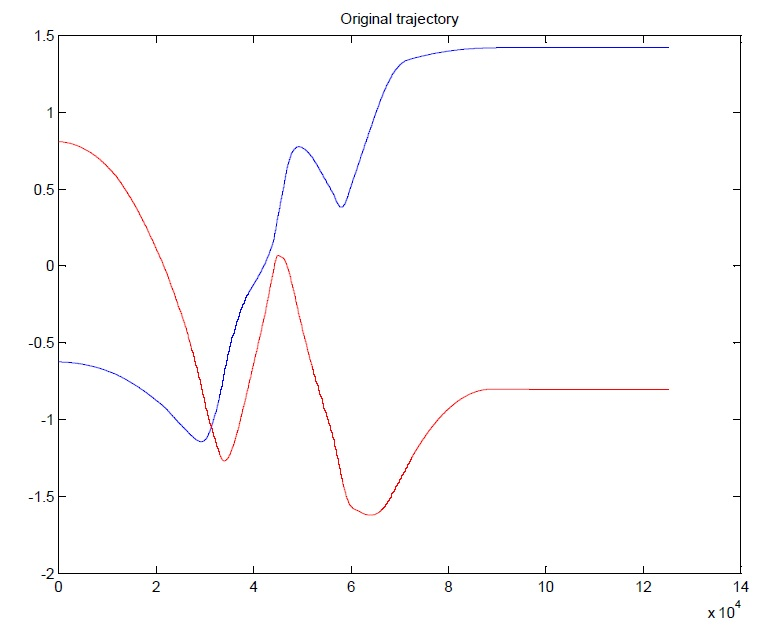
\includegraphics[width=\linewidth]{../Images/c3/sim2_traj_ori}
		\caption{Ground tracking - Original trajectory}
		\label{fig:sim2_traj_ori}
	\end{subfigure}
	~
	\begin{subfigure}[b]{0.4\linewidth}
		\centering
		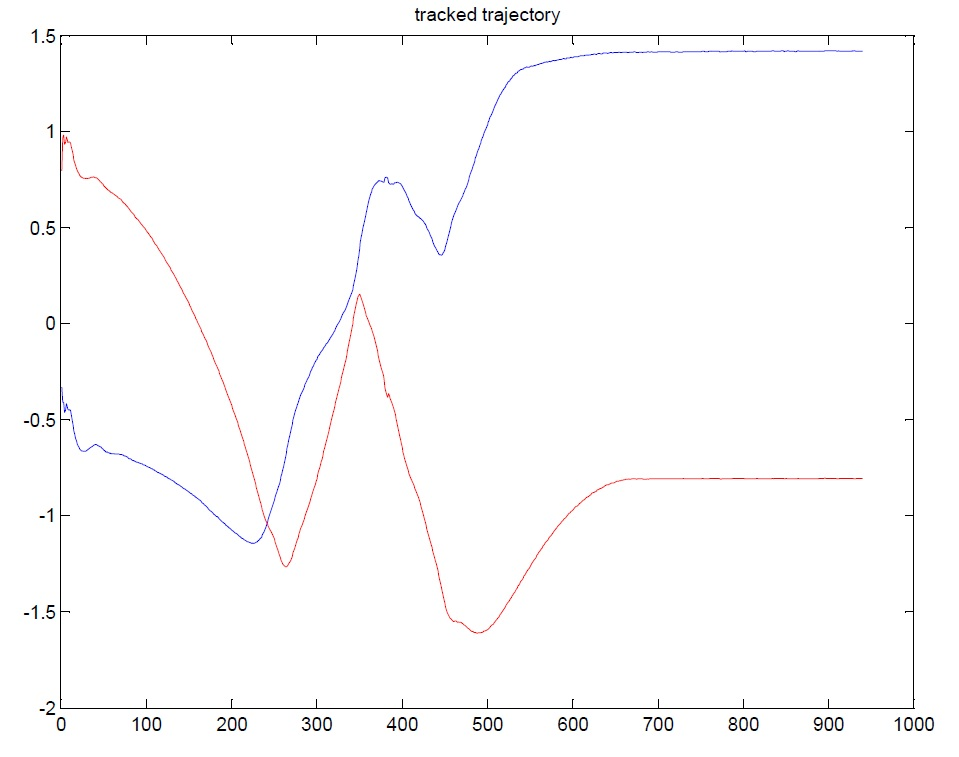
\includegraphics[width=\linewidth]{../Images/c3/sim2_traj_track}
		\caption{Ground tracking - Tracked trajectory}
		\label{fig:sim2_traj_track}
	\end{subfigure}

\end{figure}


\begin{figure}[h]
\centering
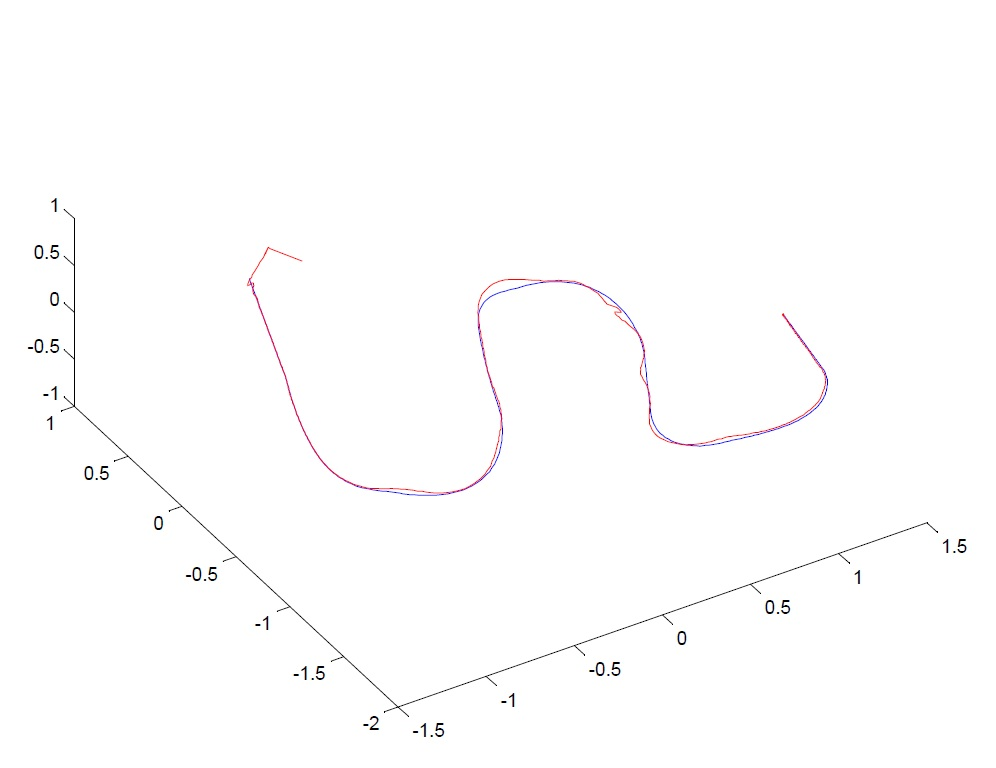
\includegraphics[width=0.7\linewidth]{../Images/c3/sim2_traj_both_3d}
\caption{Ground tracking - Oblique Camera - 3D trajectory}
\label{fig:sim2_traj_both_3d}
\end{figure}




%-------------------------------------------------------------------------------------------------------
%-------------------------------------------------------------------------------------------------------
%-------------------------------------------------------------------------------------------------------
\subsection{Stereo tracking}
\subsubsection{Set up}
This simulation is the first one with two quadcopters. The Red sphere is moving on the floor (Describing a curve) while both quad's cameras capture pictures and the on board computers (that are simulated) process them and self-command quads in order to follow the target. The cameras are also oblique (45 degrees from the previous; Figure: \ref{fig:sim3_set_up}). The speediness is the same one that in simulation 2.

\begin{figure}[h]
	\centering
	\begin{subfigure}[b]{0.4\linewidth}
	\centering
		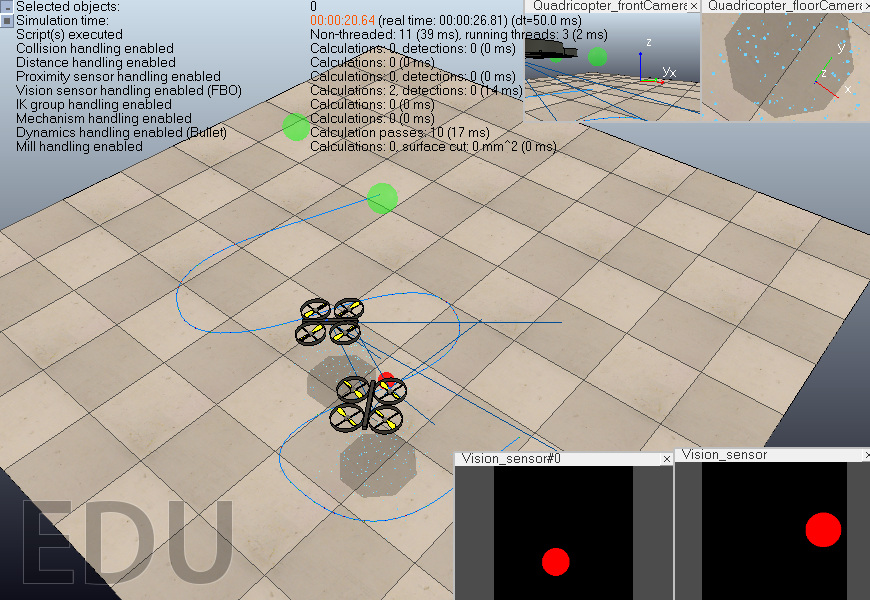
\includegraphics[width=\linewidth]{../Images/c3/sim3_set_up}
		\caption{Stereo tracking - Set up}
		\label{fig:sim3_set_up}
	\end{subfigure}
	~
	\begin{subfigure}[b]{0.4\linewidth}
		\centering
		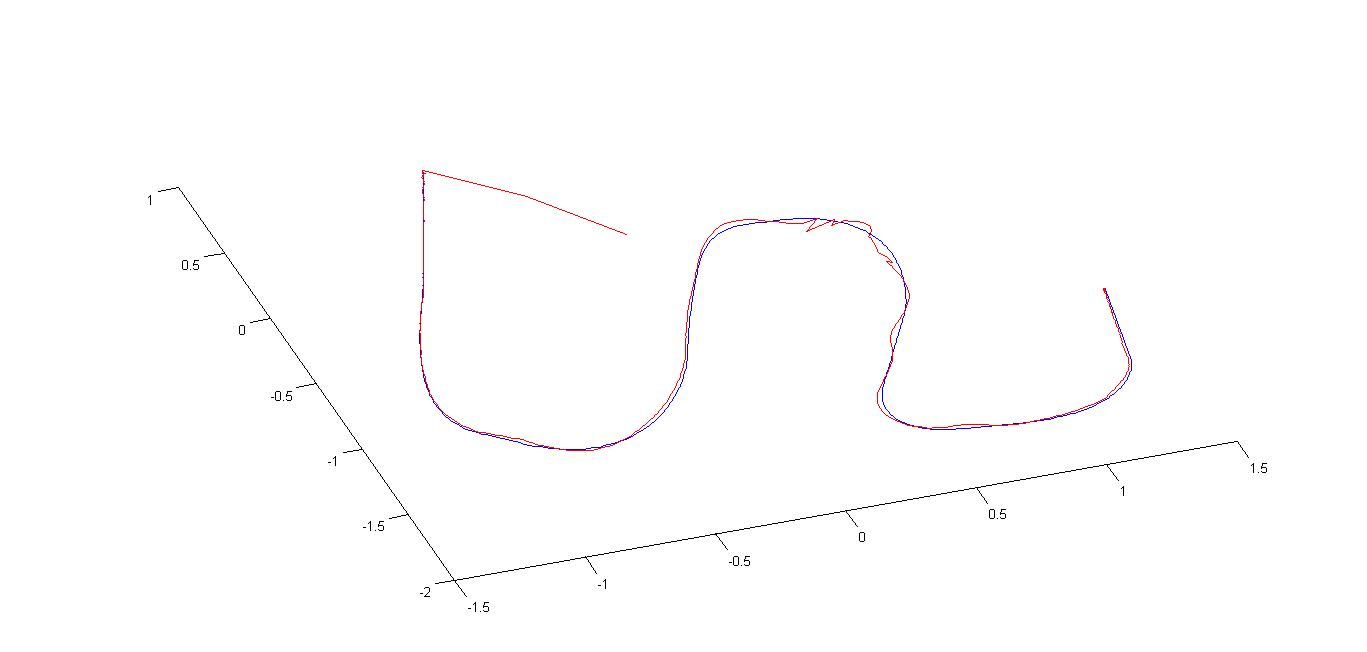
\includegraphics[width=\linewidth]{../Images/c3/sim3_traj_both_3d}
		\caption{Stereo tracking - 3D trajectory}
		\label{fig:sim3_traj_both_3d}
	\end{subfigure}
\end{figure}

\subsubsection{Test and results}

	In this simulation the results converge fastly from the initial state to the target's position. Here the max error is $\sim$ 4 cm. and medium error is $\sim$ 1 cm. Max error is found at the beginning of the second curve. That is because the target increase it's velocity considerably (And the EKF suppose a linear movement). This, together with the dynamic behavior of the quadrotors, make the path-line seems a sawtooth (Figure: \ref{fig:sim3_traj_both_3d}).
	
\begin{figure}[h]
	\centering
	\begin{subfigure}[b]{0.4\linewidth}
		\centering
		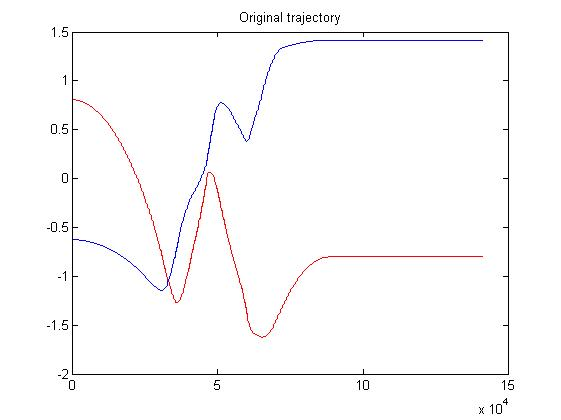
\includegraphics[width=\linewidth]{../Images/c3/sim3_traj_ori}
		\caption{Stereo tracking - Original trajectory}
		\label{fig:sim3_traj_ori}
	\end{subfigure}
	~
	\begin{subfigure}[b]{0.4\linewidth}
		\centering
		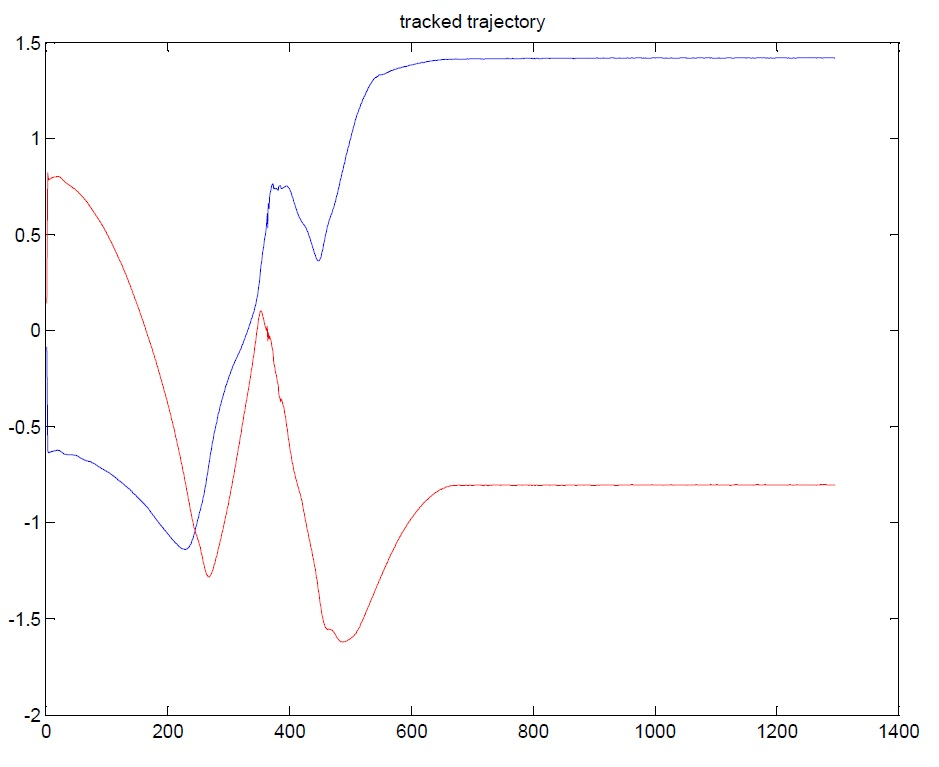
\includegraphics[width=\linewidth]{../Images/c3/sim3_traj_track}
		\caption{Stereo tracking - Tracked trajectory}
		\label{fig:sim3_traj_track}
	\end{subfigure}

\end{figure}




%-------------------------------------------------------------------------------------------------------
%-------------------------------------------------------------------------------------------------------
%-------------------------------------------------------------------------------------------------------
\subsection{Ground Tracking - Multiple targets}
\subsubsection{Set up}
 On this experiment, there is again only one quadrotor(Figure: \ref{fig:sim4_set_up}). Instead, one more target was added (Blue sphere). Both objects describe the curve, keeping their relative distance (Moving as a rigid solid, so the blue is always on the left-side of the path). the watcher's camera is also oblique (45 degrees) and spheres keeps the same speed of the previous simulation.
 
\begin{figure}[h]
	\centering
	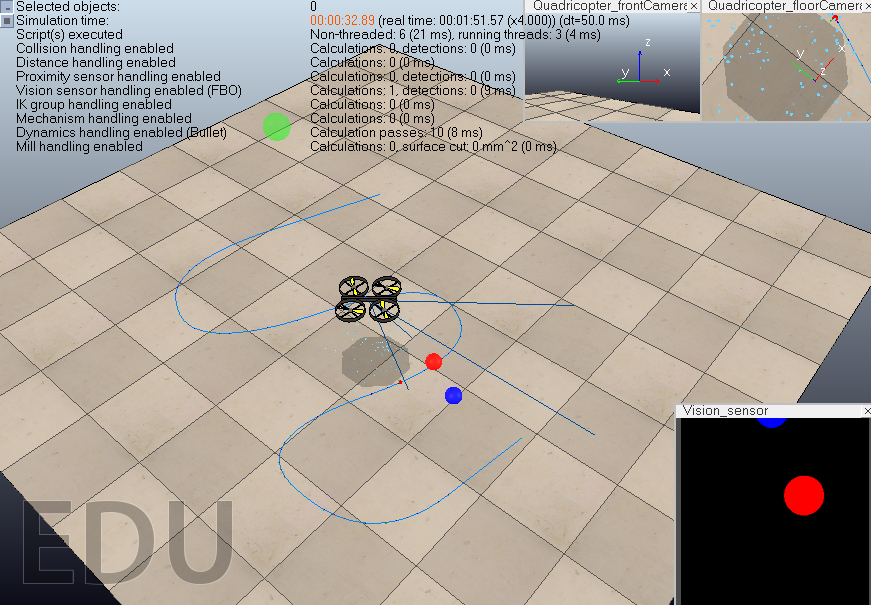
\includegraphics[width=0.7\linewidth]{../Images/c3/sim4_set_up}
	\caption{Multiple Targets - Set Up}
	\label{fig:sim4_set_up}
\end{figure}

\subsubsection{Test and results}

	Firstly, figures \ref{fig:sim4_redtarget} and \ref{fig:sim4_bluetarget} shows the X and Y coordinateguardias of the targets (Both real and estimate). Secondly, figure \ref{fig:sim4_3dtraj} shows the 3D path-lines of both red and blue spheres. \\
	
	The results of red tracking are quite good and similar to the ones explained in "Ground tracking - Oblique camera" \ref{lab:sim2_test_results}. The tracking of the blue sphere seems to be wrong. However, it is not. This deviation is due to lack of information. The camera didn't capture the whole blue sphere \ref{fig:sim4_centroid_objs}, causing an error between the centroid of the recognized part of the sphere in the image and the real one. That's why the tracked-path is always displaced a few centimeters from the real one. The maximum error is $\sim$ 20 cm and the medium is $\sim$ 6 cm.

\begin{figure}[h]
	\centering
	\begin{subfigure}[b]{0.45\linewidth}
		\centering
		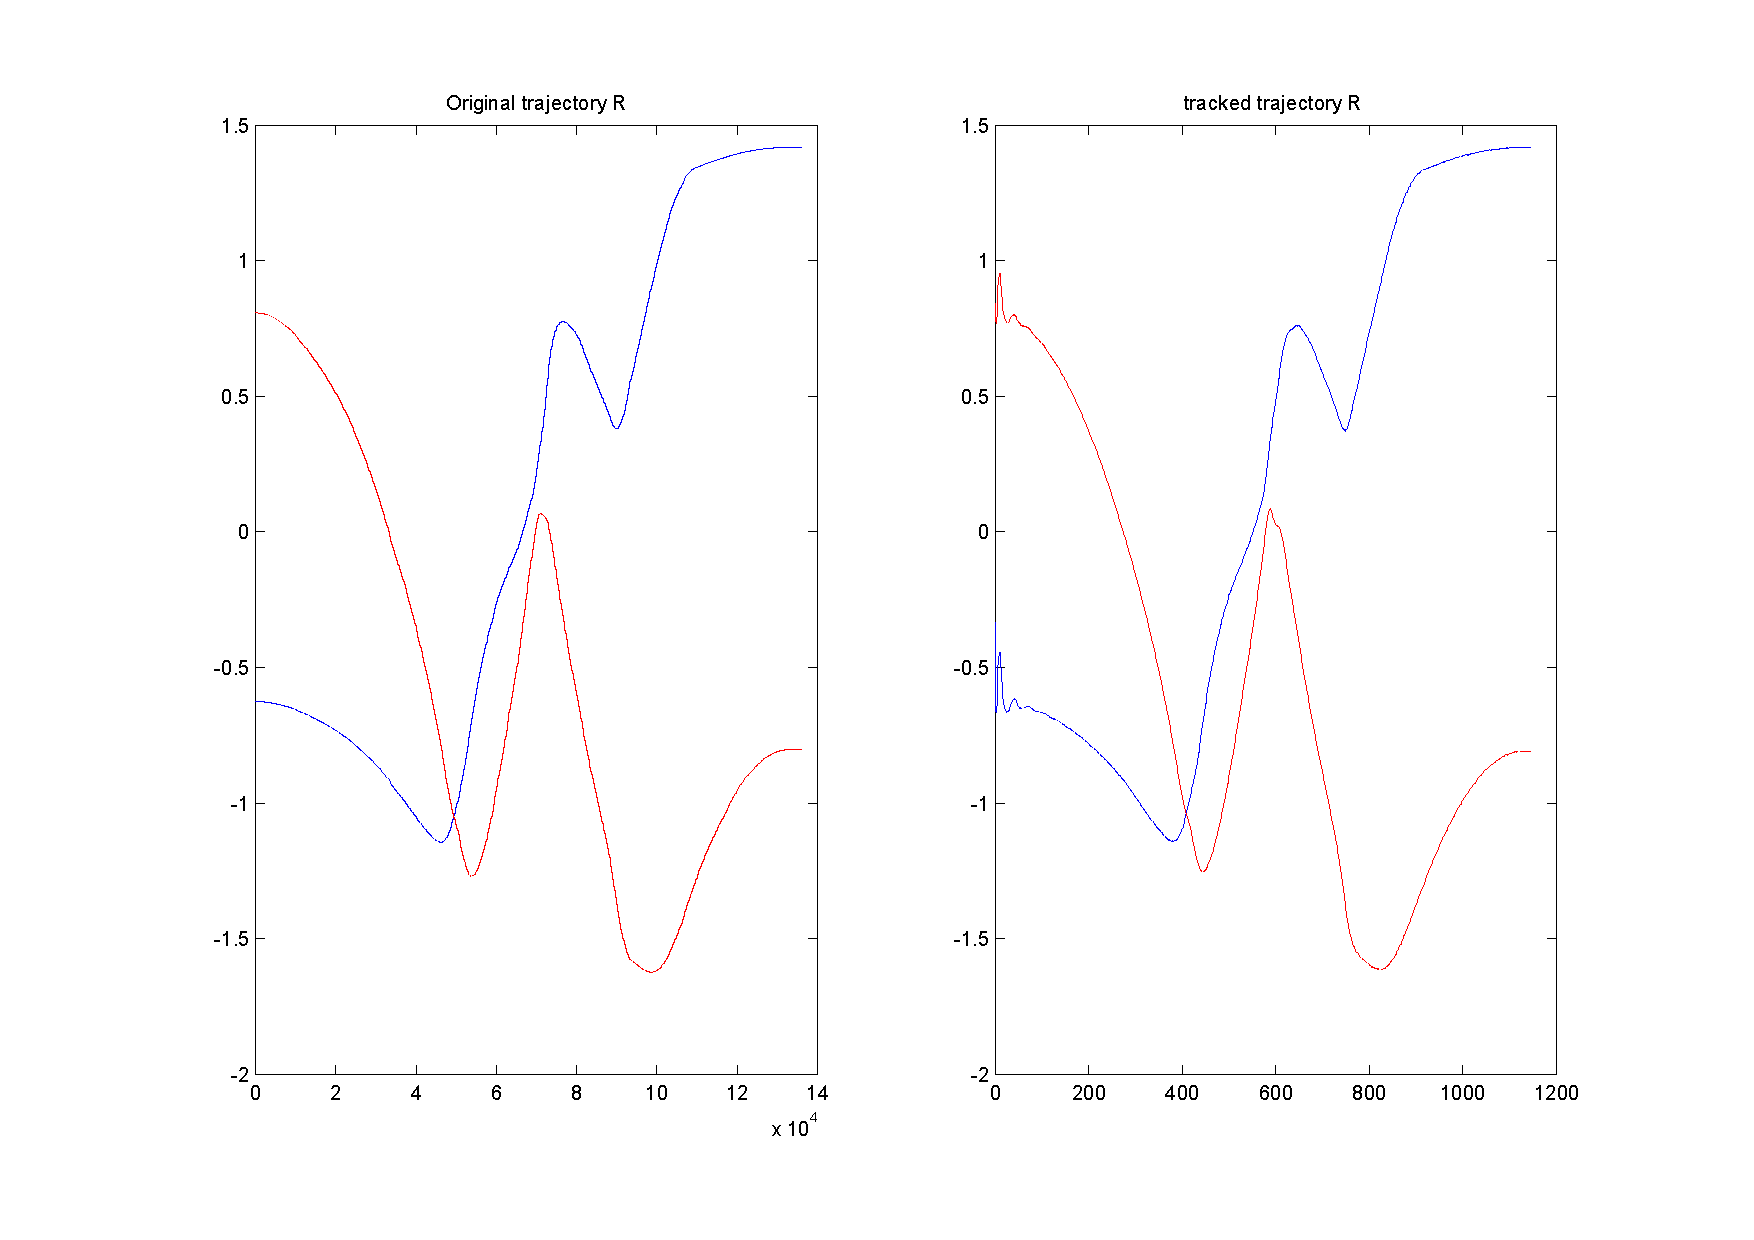
\includegraphics[width=\linewidth]{../Images/c3/sim4_redtarget}
		\caption{Multiple Targets - Red target}
		\label{fig:sim4_redtarget}	
	\end{subfigure}
	~
	\begin{subfigure}[b]{0.45\linewidth}
		\centering
		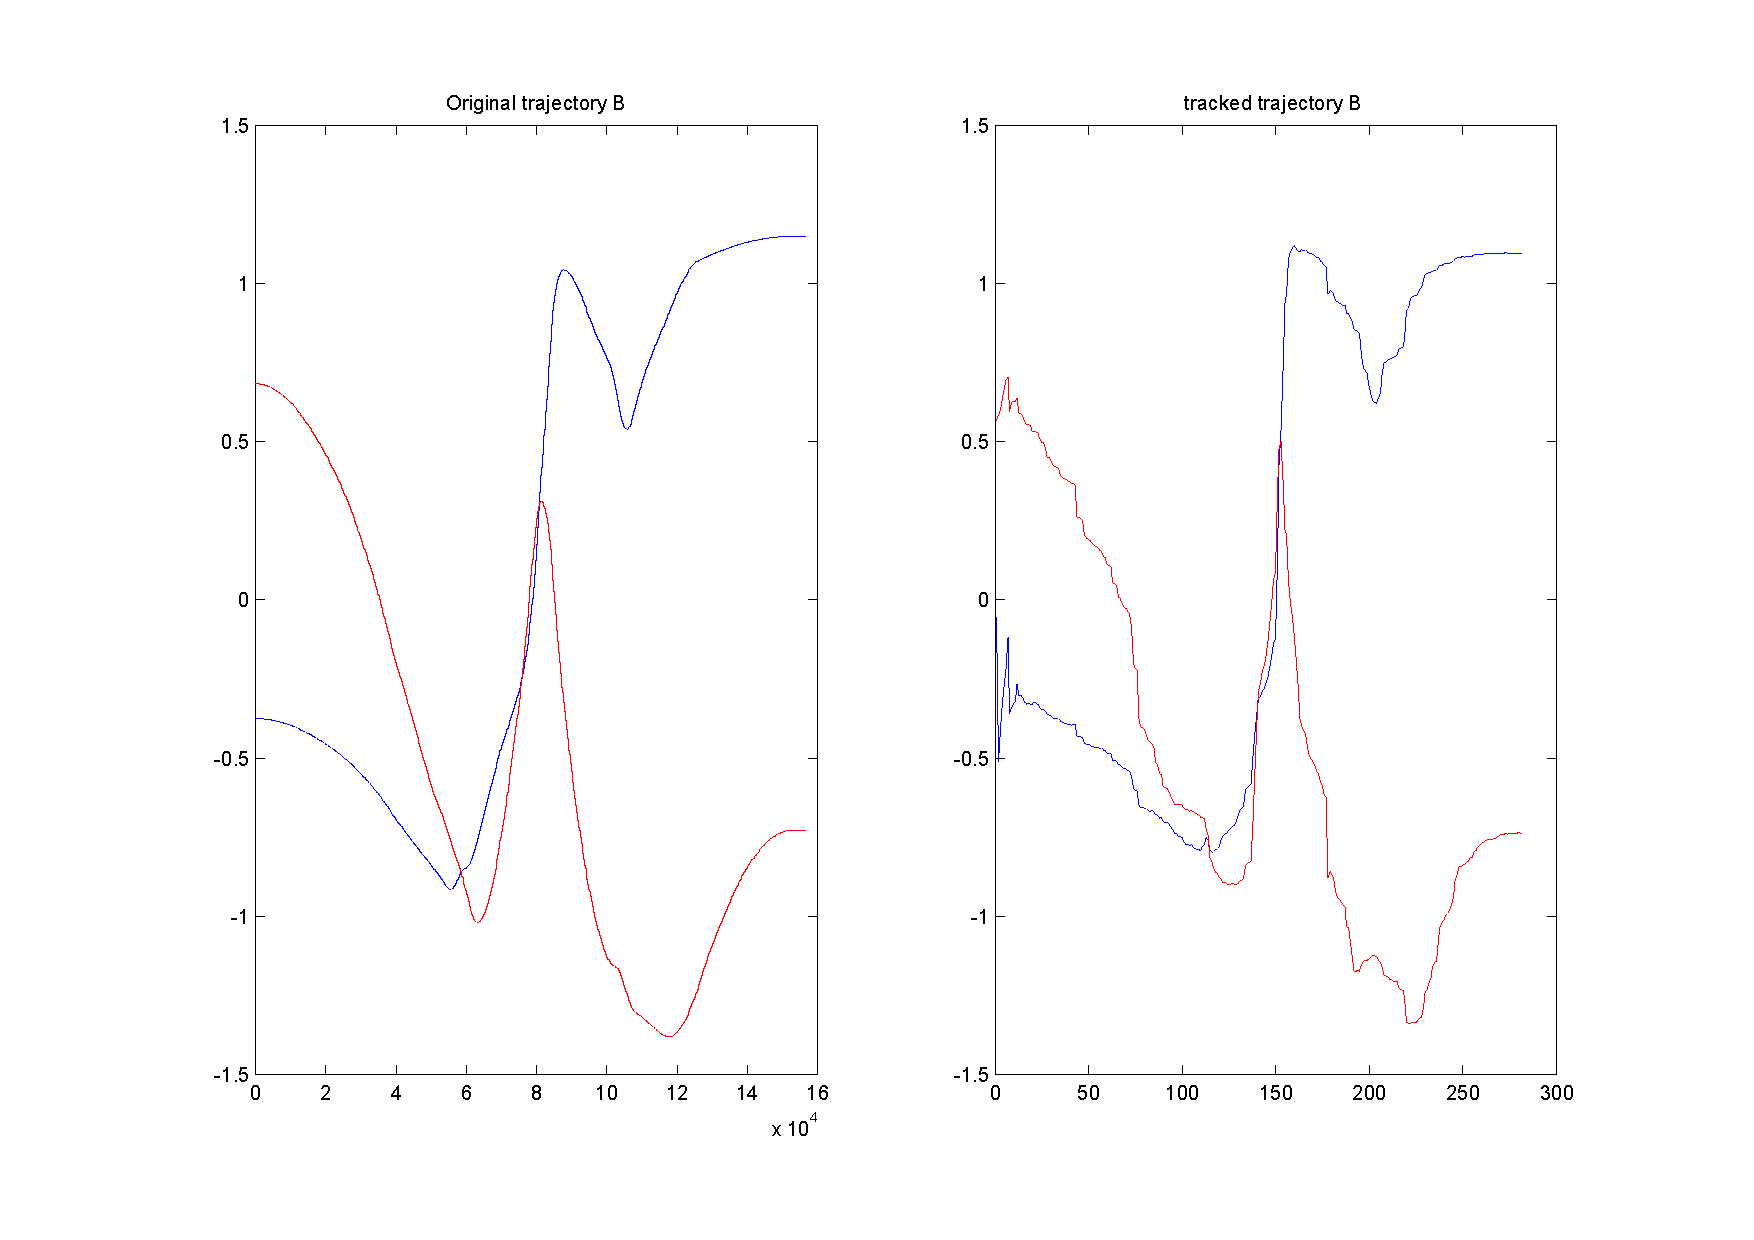
\includegraphics[width=\linewidth]{../Images/c3/sim4_bluetarget}
		\caption{Multiple Targets - Blue target}
		\label{fig:sim4_bluetarget}
	\end{subfigure}
\end{figure}

\begin{figure}[h]
	\centering
	\begin{subfigure}[b]{0.6\linewidth}
		\centering
		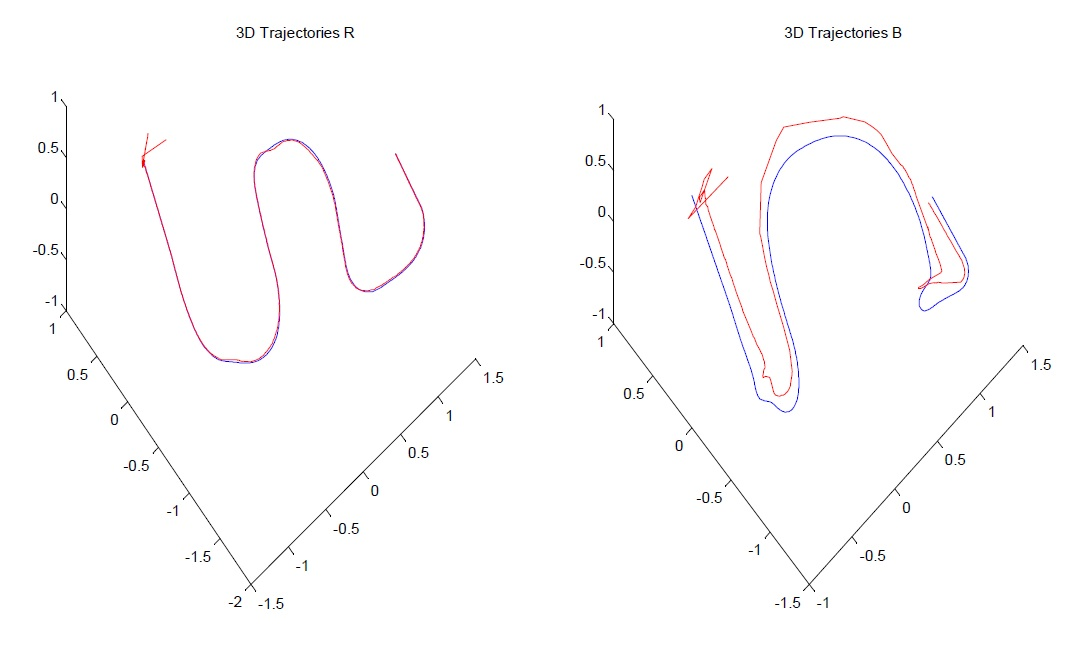
\includegraphics[width=\linewidth]{../Images/c3/sim4_3dtraj}
		\caption{Multiple Targets - 3D trajectory}
		\label{fig:sim4_3dtraj}
	\end{subfigure}
	~
	\begin{subfigure}[b]{0.2\linewidth}
		\centering
		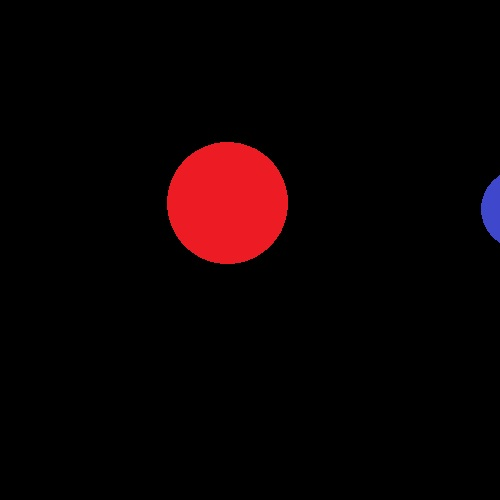
\includegraphics[width=\linewidth]{../Images/c3/sims_two_object_centroid_out}
		\caption{Multiple Targets - Objects centroids on Image}
		\label{fig:sim4_centroid_objs}
	\end{subfigure}
\end{figure}

%----------------------------------------------------------
% Chapter 4. Hardware Architecture
\chapter{Hardware Architecture}
\section{Introduction}
\section{Development Architecture}
\section{Hardware for Release}

%----------------------------------------------------------
% Chapter 5. Real tests
\chapter{Real Tests}
\section{Introduction}
\section{Hardware \& Software implementation}
\section{Results}

%----------------------------------------------------------
% Chapter 6. Conclusions
\chapter{Conclusions} \label{chap:c6_conclusions}
\section{Analyzing Results}
\section{Future Branchs}
\section{Strengths and Weakness}

%----------------------------------------------------------
\listoffigures{}

%----------------------------------------------------------
% Bibliography
\begin{thebibliography}{9}
\bibitem{JamesBruce} \textit{Fast and Inexpensive Color Image Segmentation for Interactive Robots.} James Bruce, Tucker Balch, Manuela Veloso. IROS2000. School of Computer Science Carnegie Mellon University

\bibitem{GabrielTerejanu} \textit{Extended Kalman Filter Tutorial} Gabriel A. Terejanu. IROS2000. Department of Computer Science and Engineering, University at Buffalo

\bibitem{SocketWiki} \textit{Network Socket} $http://en.wikipedia.org/wiki/Network_socket$

\bibitem{BOViL} \textit{Bardo's Open Vision Library} $https://github.com/Bardo91/BOVIL/wiki$

\bibitem{TCPIP} \textit{TCP/IP Protocol} 

\end{thebibliography}

%----------------------------------------------------------
% Ending
\backmatter

\chapter{Afterword}

\end{document}
